% --- Template for thesis / report with tktltiki2 class ---
% 
% last updated 2013/02/15 for tkltiki2 v1.02

\documentclass[english]{tktltiki2}

% tktltiki2 automatically loads babel, so you can simply
% give the language parameter (e.g. finnish, swedish, english, british) as
% a parameter for the class: \documentclass[finnish]{tktltiki2}.
% The information on title and abstract is generated automatically depending on
% the language, see below if you need to change any of these manually.
% 
% Class options:
% - grading                 -- Print labels for grading information on the front page.
% - disablelastpagecounter  -- Disables the automatic generation of page number information
%                              in the abstract. See also \numberofpagesinformation{} command below.
%
% The class also respects the following options of article class:
%   10pt, 11pt, 12pt, final, draft, oneside, twoside,
%   openright, openany, onecolumn, twocolumn, leqno, fleqn
%
% The default font size is 11pt. The paper size used is A4, other sizes are not supported.
%
% rubber: module pdftex

% --- General packages ---

\usepackage[utf8]{inputenc}
\usepackage[T1]{fontenc}
\usepackage{lmodern}
\usepackage{microtype}
\usepackage{amsfonts,amsmath,amssymb,amsthm,booktabs,color,enumitem,graphicx}
\usepackage[pdftex,hidelinks]{hyperref}

\usepackage{subfigure}
\usepackage[textsize=tiny, disable]{todonotes}
\usepackage{multirow} 
\usepackage{array}
\usepackage{setspace}
\usepackage{morefloats}


% Automatically set the PDF metadata fields
\makeatletter
\AtBeginDocument{\hypersetup{pdftitle = {\@title}, pdfauthor = {\@author}}}
\makeatother

% --- Language-related settings ---
%
% these should be modified according to your language

% babelbib for non-english bibliography using bibtex
\usepackage[fixlanguage]{babelbib}

% add bibliography to the table of contents
\usepackage[nottoc]{tocbibind}

% --- Theorem environment definitions ---

\newtheorem{thm}{Theorem}
\newtheorem{lem}[thm]{Lemma}
\newtheorem{cor}[thm]{Corollary}

\theoremstyle{definition}
\newtheorem{definition}[thm]{Definition}

\theoremstyle{remark}
\newtheorem*{remark}{Remark}


% --- tktltiki2 options ---
%
% The following commands define the information used to generate title and
% abstract pages. The following entries should be always specified:

\title{Theory and practice of rapid elasticity in cloud applications}
\author{Mika Majakorpi}
\date{\today}
\level{MSc Thesis}
\abstract{

This thesis is a study of the theory of scalability and its application in an
infrastructure as a service (IaaS) cloud context. The cloud based utility
computing paradigm is presented along with how scalability principles are
applied in the cloud. The differences of scalability in general and the cloud
concept of elasticity are discussed.

A \textit{quality of elasticity (QoE)} metric is developed to facilitate factual
discussion and comparison of different cloud platforms' elasticity capabilities
and the effectiveness of elastic scaling strategies. The metric is based on
business requirements expressed as \textit{preference functions} over a set of
lower level metrics. Multi-criteria analysis is applied to these possibly
conflicting preferences to arrive at a unified value of \textit{utility} based
on weighting the sum of the preferences. QoE reflects the utility of the system
over time.

The concept of an elasticity controller application is presented and a prototype
implementation described in order to exercise the QoE metric. Two load testing
scenarios are executed against a simple test application whose deployment is
managed by the prototype controller. The elastic scaling behavior of the system
is analysed in terms of the QoE results to confirm the prototype is functional
and to find areas of improvement.

}

% The following can be used to specify keywords and classification of the paper:

\keywords{cloud computing, scalability, elasticity}
% classification according to ACM Computing Classification System (http://www.acm.org/about/class/)
% This is probably mostly relevant for computer scientists
\classification{\protect{\ \\
\textbf{Networks $\rightarrow$ Cloud computing} \\
\textbf{Software and its engineering $\rightarrow$ Software performance} \\
\textit{Computer systems organization $\rightarrow$ Reliability} \\
General and reference $\rightarrow$  Metrics \\
}}
%→
% If the automatic page number counting is not working as desired in your case,
% uncomment the following to manually set the number of pages displayed in the abstract page:
%
% \numberofpagesinformation{16 pages + 10 appendix pages}
%
% If you are not a computer scientist, you will want to uncomment the following by hand and specify
% your department, faculty and subject by hand:
%
% \faculty{Faculty of Science}
% \department{Department of Computer Science}
% \subject{Computer Science}
%
% If you are not from the University of Helsinki, then you will most likely want to set these also:
%
% \university{University of Helsinki}
% \universitylong{HELSINGIN YLIOPISTO --- HELSINGFORS UNIVERSITET --- UNIVERSITY OF HELSINKI} % displayed on the top of the abstract page
% \city{Helsinki}
%
%\doublespacing
%\singlespacing
\onehalfspacing
\setlength{\parindent}{0mm}
\setlength{\parskip}{1ex}

\begin{document}

% --- Front matter ---

\maketitle        % title page
\makeabstract     % abstract page

\tableofcontents  % table of contents
\newpage          % clear page after the table of contents


%\newenvironment{acknowledgements}%
%    {\cleardoublepage\thispagestyle{empty}\null\vfill\begin{center}%
%    \bfseries Acknowledgements\end{center}}%
~\\[10\baselineskip]    
%{\vfill\null}
        \begin{center}
        \textit{For Rashmi}\\
        \textit{Your resolve inspires me}
        \end{center}

%\listoffigures
%\listoftables

\listoftodos
\newpage

% --- Main matter ---

\section{Introduction}

Computer science is a discipline built on layers upon layers of abstraction. We
build entire worlds out of combinations of binary states. When complexity
increases over a practical threshold, we apply another abstraction layer and
continue until we face another technological or conceptual limit. Progress
happens when new abstractions emerge either leveraging existing ones or
replacing and simplifying them.

The context of this thesis is scalability in cloud computing, a recent
abstraction built on virtualization and distributed computing~\cite{handbook}.
Technologies related to cloud computing accelerate the provisioning of computing
resources by several orders of magnitude compared to a non-virtualized process.
Resources are provided to users as virtual units which draw on a pool of
distributed physical resources collectively called a cloud. The lead time to
acquire a virtual server instance is measured in seconds or minutes instead of
days or even weeks~\cite{elasticsiteMarshall2010}. When the server is no longer
needed or during times of inactivity the resources reserved for the server are
allocated to other virtual resources or released back to the cloud as free
capacity. This flexibility drives down costs and provides the possibility for
new kinds of agile ICT.

The apparent unlimited supply and instant delivery of resources has inspired
researchers to consider cloud computing as a utility similar to water and
electricity~\cite{Buyya2009a}; It’s ubiquitously available and billed based on
usage. The ease at which cloud resources can be provisioned makes it possible to
run applications with an adjustable amount of server instances depending on the
current or anticipated usage level of the application. This flexibility and the
speed with which the deployment can be adjusted have enabled e.g. web
applications to scale from a handful of concurrent sessions to millions~\cite{
cloudberkeleyviewacm} and back without committing to a large amount of computing
resources which would remain deployed but unused during periods of low usage. A
deployment capable of serving millions of users is understandably expensive to
maintain, but the cloud approach with its prevalent pay per use pricing enables
such scenarios to be realized without large upfront investment in computing
resources as would be the case with dedicated hardware servers.

The ability of an application deployment on a cloud platform to change in size
dynamically at runtime is referred to as elasticity or rapid elasticity~\cite{
nistdefinition}. This capability to automatically scale the deployment in
(smaller) or out (larger) depending on current demand is a major factor in
the hype and success~\cite{cloudberkeleyviewacm} of cloud platforms in recent years.

The goal of this thesis is to explore the theory and practice of rapid
elasticity. The concept of quality of elasticity is developed and put to test
using a prototype implementation of an elasticity controller~\cite{VRB11}, a
piece of cloud infrastructure software whose responsibility is to decide on and
implement cloud provisioning actions. The focus is on infrastructure as a
service (IaaS) clouds and the provisioning of virtual machines in such clouds.
The elasticity controller concept is a step towards a more service oriented
cloud offering. Rather than provide infrastructure with an interface modeled
exactly after the operations performed on IaaS VMs, a service-oriented approach
aims to provide more abstract interfaces which address the cloud customer’s
problem domain rather than the cloud provider’s. This includes e.g. cross-cloud
capabilities~\cite{frominfratoservice}.

The thesis is structured as follows. Chapter~\ref{sec:scalability} discusses the
different forms of scalability in system and software architectures.
Chapter~\ref{sec:cloudscalability} presents scalability in cloud context.
Chapter~\ref{sec:elasticity} discusses the theory of elastic scaling and
develops a metric, quality of elasticity, for it. Architectural patterns to take
full advantage of elasticity are also presented in this chapter.
Chapter~\ref{sec:elasticScalingPrototype} presents an elasticity controller
prototype along with its requisite monitoring infrastructure used in the thesis
to put the theory to test in practice.

Results of two test load scenarios are presented in chapter~\ref{sec:results}. The
two scenarios compare quality of elasticity under a gradually growing load and a
sudden spike of load. Areas of further development are discussed based on the
findings of the tests. Finally, chapter~\ref{sec:conclusion} concludes the thesis.

\subsection{Cloud computing terminology} Cloud computing
is often referred to quite vaguely as a massively scalable model for
infrastructure services in information technology. As academic research and
practical use grows, more and more terms and conceptual frameworks related to
cloud computing are emerging, some of them short lived or focused on marketing.
Published taxonomies~\cite{Hofer2011taxonomy} offer a snapshot to a fast moving
target. The following terms for deployment models and abstraction levels are
fixed in common usage~\cite{nistdefinition}~\cite{handbook} and essential to
understanding the scope of cloud computing.

A cloud is \emph{public} if it is available for the general public to access and
\emph{private} if it is only available internally to some organization or
selected group of organizations. Obvious differences from a cloud user’s
perspective are the location of data and management of physical resources on
which the virtualization environment is built. \emph{Hybrid} clouds are a
combination of the above such that a private cloud is bridged to another private
or public cloud. They remain functionally independent but the private clouds
gain benefits in tolerance against hardware failure and resource exhaustion as
workload (i.e. virtual machines) can be shifted elsewhere in case of a shortage
of capacity. Such expansion of a private cloud is called
cloudbursting~\cite{nistdefinition}. When a private cloud is the actor in
cloudbursting, it is considered functionally transparent to the users of the
cloud. The cloud user has a single interface towards the cloud which handles
bursting behind the scenes. Bursting may also be implemented outside any cloud
infrastructure layer, closer to the application. In this case bursting is
typically handled by an application controller component in charge of elastic
scaling (elasticity controller).

Varying the size of a deployment or the amount of resources reserved for a task is called scaling. Adding more resource instances (e.g. a virtual machine) is referred to as \textit{scaling out}. Decreasing the amount of resource instances is called \textit{scaling in}. This is in contrast to modifying the capabilities of an existing resource instance, which is referred to as \textit{scaling up} for more and \textit{scaling down} for less.

Customers can benefit from clouds at different levels of service. The simplest
case for a customer is using cloud deployed \emph{software as a service (SaaS)}
without having to consider any operative aspects of the software. Gmail is
an example in this category. Google operates the service supposedly deployed on
their private cloud infrastructure and customers merely log in to the service
and use it over the Internet. Moving down to the next level of service,
customers can deploy their own applications to \emph{platform as a service
(PaaS)} clouds like Heroku, Microsoft Azure or Google App Engine. The service
provided is a platform for applications with related application programming
interfaces (APIs) and services for managing and monitoring the deployment. A
PaaS cloud enables customers to focus on the application instead of
infrastructure at the cost of losing control and ownership of it. One further
level down, \emph{infrastructure as a service (IaaS)} clouds enable customers to
provision virtualized infrastructure resources (virtual machines, storage,
network) to build their own infrastructure, platform and application. IaaS gives
the most control on the deployment, but requires considerably more management
compared to the other service levels.

Cloud service levels form a hierarchy with infrastructure at the bottom, a
platform deployed on the infrastructure and software on the platform offered as
a service to customers. A new service or application may be built by leveraging
any of these service levels. For example, the Heroku PaaS platform uses Amazon’s
EC2 infrastructure and an application deployed on Heroku will then complete the
stack. On the other hand, an application could simply be deployed on EC2,
skipping the PaaS layer, if it was deemed beneficial to gain additional control
of the stack down to virtual infrastructure. Starting at a lower abstraction
level increases the responsibilities of the application or organization
operating it to include infrastructure or platform management as well as
managing the application.

Ultimately all deployment models and service levels are meant to provide
scalable computing resources to customers. How to best benefit from scalability and what it actually means in each case is up to the customer.

\section{Scalability}
\label{sec:scalability}

Scalability is one of the elusive ``-ilities'' in information systems, a quality
attribute whose importance for an application deployment is clearly demonstrated
when the usage of a system grows and resource demands increase. Yet it is
hard to pin down exactly what scalability means in each discussion of
it~\cite{ScalabilityHill1990}.

Computing resources are limited and eventually any system which grows in data or
usage will saturate the resources available to it. The system may then also end
up needlessly large or expensive in case resource requirements decrease
afterwards. The resources in question may be e.g. processing capacity for
computationally intensive systems or storage capacity for data intensive
systems. Network capacity is a notable scalability point in distributed systems.
Structural scalability concerns the internal design of a system and how the
design lends itself to growth or shrinking of the system’s data model or, for
example, its deployment.

\subsection{Dimensions}

%The vocabulary: scale up, out, down, in wrt vertical, horizontal  

Scalability has multiple dimensions as illustrated in
figure~\ref{fig:scalabilityDimensions}. Scaling is said to be \emph{vertical} if
the scaling point or points in question are internal to a server. For example,
the amount of RAM available to a specific server or its CPU speed is a vertical
scaling point in terms of that server. A vertically scaled system remains
logically equivalent in the process of scaling. Scaling this way is
straightforward as software requires no changes to take advantage of further
resources on a system. In contrast, adding more server instances,
\emph{horizontal} scaling, is a more coarse grained operation and requires
software to be written specifically to leverage the multiple servers by running
tasks in parallel~\cite{handbook-scaling}.

%The following paragraph is possibly better suited for the rapid elasticity or
%elastic architectures chapter? 

Switching to a higher level of abstraction in system design changes the
viewpoint from horizontal to vertical. Horizontal scaling of nodes in a server
cluster or cloud can be considered vertical scaling from the viewpoint of the
utility provided (e.g. processing capacity) by it to a higher level system using
it as a component. This is how infrastructure as a service (IaaS) and platform
as a service (PaaS) scaling viewpoints differ. Horizontal IaaS virtual machine
scaling is vertical platform capacity scaling from the viewpoint of an
application deployed on a PaaS cloud where the platform manages the
infrastructure.

The vertical dimension gets exponentially more expensive as the system size
increases. The scaled system needs to be changed to a more capable type of
server as the need for more resources increases past what the current server can
physically support. This scaling path eventually leads to mainframes and
supercomputers. The limits for horizontal scaling, on the other hand, are
traditionally in the domain of data centers and the amount of servers that can
fit on their racks. Horizontal scaling has been very common in Internet
architectures since the early days of the network, but recently virtualization
has made vertical scaling an important option to consider as well~\cite{VRB11}.
With vertical scaling, system configuration can be adjusted dynamically at
runtime in a matter of seconds, which is faster than the minute-or-two time
frame of horizontal scaling in a cloud. A combination of both scaling dimensions
can be used to implement a fine grained scaling solution.

Cloud computing pushes both scaling dimensions past their traditional
boundaries. Hybrid clouds and cloud interoperability make it possible to scale
out a system past the boundaries of data centers and cloud providers. The
network becomes the limiting factor here as the communication between nodes in a
system needs to be transmitted between clouds over the Internet.

A third dimension to consider is \emph{structural scalability} which has to do
with the behavior of a piece of software as its data model, amount of data or
amount of tasks to execute varies in size~\cite{handbook-scaling}. A requirement
for scalable software is to be internally efficient in terms of the asymptotic
time and space complexity of its algorithms~\cite{algorithmBook} and
additionally support parallel processing in terms of tasks and
data~\cite{foundationsOfParallelBook}.

\begin{figure}[htbp]
	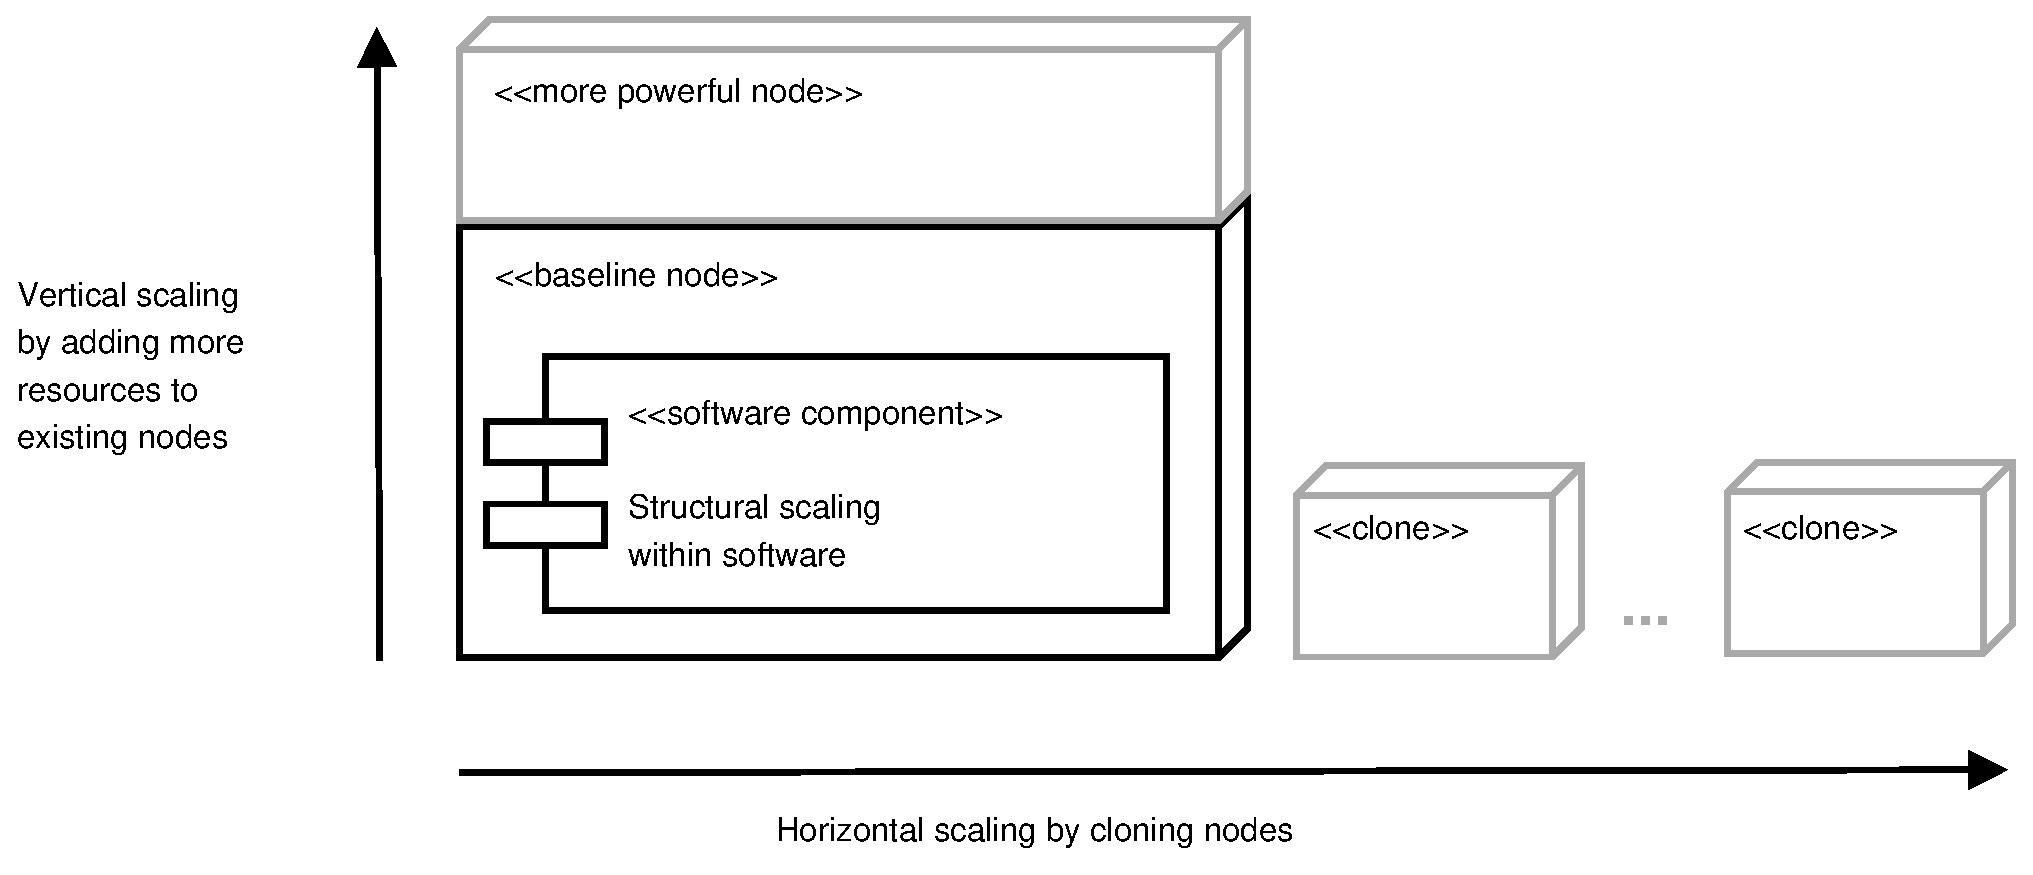
\includegraphics[width=\textwidth]{images/scalingDimensions}
	\caption{Three dimensions of scalability}
	\label{fig:scalabilityDimensions}
\end{figure}

Task parallelism is a feature of software systems which are capable of
simultaneously executing multiple tasks on the same or different data. A serial
program, in contrast, must proceed with a single task at a time. Task parallel
software lends itself well to horizontal scaling as separate tasks can be
executed on distributed nodes of a system. Vertical scaling, on the other hand,
can be applied to adjust the performance of each task independently.

Data parallelism is the capability of a software system to perform the same
operation in parallel to different instances of data. In distributed systems, a
large computing task is typically split into multiple independent tasks which
can be executed on separate server nodes simultaneously without communication
between them. Results of the split tasks are then sent back to a controller
which combines them and computes the final result. This was done in large
scale already back in 1999 with the Seti@Home project. Since then millions of
ordinary computer users have donated CPU time to search for extraterrestrial
intelligence by running an application which analyzes pieces of a large set of
radio telescope data~\cite{Korpela2001}\cite{setiathomewebsite}. More recently
Google and e.g. the open source distributed database Hadoop have made use of the
MapReduce programming model~\cite{handbook-mapreduce} for distributed data
parallel computing.

Structural scalability is closely related to the horizontal scaling dimension.
To take full advantage of horizontal scaling, the application has to support
parallel execution and minimize synchronization between the parallel threads of
execution. Depending on the use case, parallelism can be either task or data
based, but in both cases the notion of parallelism has to be built in to the
application.

\subsection{Tradeoffs}

Scaling a system is not without its negatives. Vertical scaling gets expensive
at an exponential rate when the system grows in available resources. Horizontal
scaling increases complexity of coordination between distributed nodes.
Structural scaling requires algorithm and data model design to fit the chosen
scaling mechanism.

Advances in computer science and technology have reduced the impact of these
tradeoffs from what it used to be with older technology. Virtualization and
dynamic provisioning of virtual machines have made it possible to use computing
resources more efficiently in a modern data center. High capacity servers are
not kept idle waiting for spikes in system load. Virtual resources can be
allocated dynamically based on demand at any given time. Nevertheless, for
vertical scaling, the cost is still the definitive tradeoff.

With horizontal scaling, a common tradeoff point is the need for communication
between nodes in a distributed system. If such communication can be avoided or
minimized, the software scales well; Adding servers does not cause excessive use
of network bandwidth and the benefit of additional servers does not decrease as
the amount of servers increases. This could happen due to increased processing
needed for keeping the system's increasingly complex state synchronized. For
data parallel computations, the MapReduce model enables this on a massive scale
but requires algorithms to fit its mold with two distinct phases, \emph{map} and
\emph{reduce}~\cite{handbook-mapreduce}. The map phase distributes data to
mapper nodes where it is processed. Intermediate results from the map phase are
fed to reducer nodes for another round processing which ends with the final
result. Both of the steps can be processed in parallel on distributed systems.
The model clearly requires a specific approach to algorithm implementation in
order to take advantage of parallel computation and is only applicable to
structurally similar problems which can be expressed in terms of the map and
reduce functions.

Task parallel software can get congested due to synchronized access to common
data. ACID (Atomicity, Consistency, Isolation, Durability) transactions are
inherently serial in nature so a shared relational database, for example,
quickly emerges as a bottleneck for scalability. To remedy this, databases can
be scaled by applying various techniques such as
sharding~\cite{scalableDataStores}. Need for ACID transactions should also be
scrutinized. Many highly scalable systems make do with the BASE (Basically
Available, Soft state, Eventually Consistent) consistency model in favor of the
more strict ACID model~\cite{tivitbestpractices}\cite{VRB11}\cite{Buyya2010intercloud}.

When scaling in, the tradeoff is with ensuring performance and
reliability while minimizing cost. When a deployment is at its minimum size,
it’s difficult to reliably react to increased load without false positives and
try to keep the application responsive. Scaling out to accommodate the
load will take some time, so the decision should be made early enough to keep
the application responsive during the scaling activity~\cite{Roy2011}. Ensuring
performance, reliability and fault tolerance as required by e.g a service level
agreement~\cite{Funika2011}\cite{Iqbal2011} sets limits for the minimum system
configuration. A capacity buffer of appropriate size has to be kept to allow
time for scaling activities.

At code level, in addition to the need for communication between horizontal
nodes, tradeoffs are made between the asymptotic complexity of algorithms in
terms of CPU time or data storage space needed for execution. System design
principles are of key importance to minimize the impact of scalability
tradeoffs.

Scalability should be considered in context. Discussing e.g. only the CPU
capacity of a system is a moot point if the system becomes overly complex or
expensive to maintain due to the increase in computational capacity. Designing a
system with one scalability factor in mind may reduce scalability in terms of
other factors. Tradeoffs like these are important to understand when designing
systems. The relative importance of scalability factors can be derived from the
requirements of the system in question. By going after the most important
factors, the utility (performance maintained by scaling which the stakeholders
experience as a tangible benefit)~\cite{Duboc2007} of the scaling effort is
the highest.

Scalability can be analyzed as a multi-criteria optimization problem where, given
the priorities of the system in question, different scaling strategies will
perform differently as the system grows. Multi-criteria analysis will help to
choose the correct scaling factors from both technical and stakeholder benefit
viewpoints as shown by Duboc in her work on the subject~\cite{Duboc2007}.
Choosing the strategy with the most utility for the system’s stakeholders should
be the goal.

\subsection{Bounds}
\label{sec:scalabilityBounds}

%speedup, amount of work done in same time, asymptotic complexity 

Scalability analysis in the design phase of a system can save effort and costs
during a system’s lifetime as changes are easiest and cheapest to make in the
beginning. Any real system will have its bounds set by its environment and
stakeholders through functional and non-functional requirements. Some
requirements are harder to meet than others and an understanding of the laws of
scalability helps in managing expectations and succeeding in system
implementation. This chapter presents basic laws of scalability to establish the
limits within which scalability engineering takes place.

Typically a portion of any computation is not parallelizable. The size of this
portion determines the lower bound in terms of execution time for a program
according to Amdahl’s law~\cite{amdahlslaw}. The law can be expressed as a
function which gives the maximum speedup $S$ that can be achieved with $N$ nodes
working in parallel,

\begin{equation}
S(N) = \frac{1}{(1-P)+\frac{P}{N}},
\label{eq:amdahlslaw}
\end{equation}

where $P$ is the portion of the program that can be executed in parallel and
conversely $(1-P)$ the serial portion. As $N$ tends to infinity, the speedup
tends to $1/(1-P)$. 


For example, if a given computation has a serial part which is 10\% of the
complete computation, then the benefit of increasing parallelism for the
remainder of the computation will tend towards zero as the number of parallel
nodes increases. The upper bound for $S(N)$ in this case is 10. The computation
can be sped up at most by a factor of 10 regardless of the amount of parallel
processors introduced to the system. This along with other values of $P$ are
illustrated in figure~\ref{fig:amdahlsLaw}. 

Before reaching the theoretical limit given by Amdahl's law, typically a
practical limit for evenly dividing $P$ into parallel tasks or data sets would
be reached. This implies that software design level structural scalability is
very important in order to keep the non-parallelizable code to a minimum.

\begin{figure}[h!]
	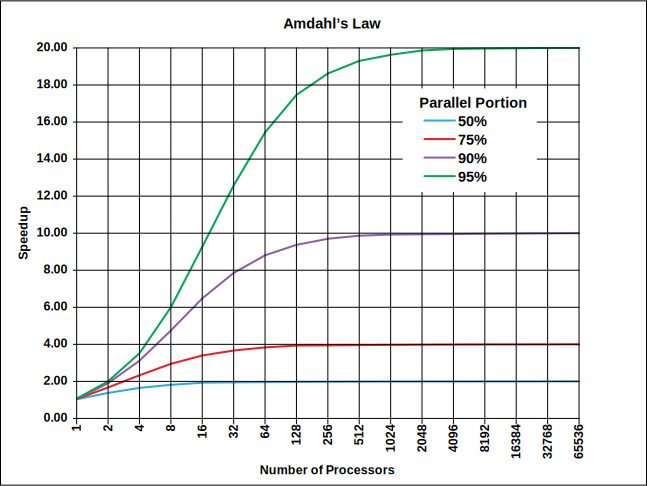
\includegraphics[width=\textwidth]{images/AmdahlsLaw}
	\caption{Amdahl's law states that the maximum speedup of a program when running 
	it on multiple processors is limited by the portion of the program that can be 
	run in parallel. (Image source: Wikimedia Commons~\cite{amdahlslawimage})}
	\label{fig:amdahlsLaw}
\end{figure}

Amdahl’s law underlines the importance of algorithmic optimization to maximize
the speedup achievable with parallel processing. However, although the benefit
of adding more parallel nodes tends to zero, the processing capacity of each of
the nodes does not of course diminish in the process. In fact, the entire array
of parallel nodes is idle for $1-P$ percent of the execution. To make efficient
use of a horizontally scalable system, the problem therefore needs to be of a
nature which benefits from a large number of $N$. That is, the portion of
inherently serial code $1-P$ needs to be minimized and the problem needs to be
divisible to $N$ or more parallel parts.

Dividing a fixed set of data or tasks can only be done in a limited number of
practical ways. Amdahl’s law assumes a static size and even division for data
over $N$ nodes and gives the maximum proportional speed but does not consider
that more data or tasks can be processed in the same time. In practice, the
benefit of parallel processing is larger given a problem with dynamic data or
task set size. Having more data or tasks is key to being able to split them $N$
ways. With virtualization, $N$ can also be adjusted to fit the input size.
\todo{could also discuss efficiency of parallel processing, E = S/N.}

Gustafson’s law~\cite{gustafsonslaw} shows that parallel processing is efficient
given the right kind of problem. It assumes the serial fraction of computation
$\alpha=1-P$ is static while the divisible amount of data or tasks grows evenly
with the amount of parallel nodes $N$. The speedup according to the law is then

\begin{equation}
S(N) = N - \alpha(N-1).
\label{eq:gustafsonslaw}
\end{equation}

In practice $\alpha$ will also grow due to overhead caused by increased
parallelism, but as long as the overhead is insignificant, Gustafson’s law shows
that scaling horizontally is efficient up to large numbers of $N$ if the data or
task size grows with the system. This is illustrated in figure~\ref{fig:gustafsonsLaw}.

In contrast to Amdah’ls law, Gustafson shows that parallel computing in a
dynamic environment (data divided into parts equal in amount to that of
computing nodes) scales very well. Recently multicore processors have brought
more possibilities to architecting scalability~\cite{amhdalmulticore} but the
basic principles from the 1960s still apply for computations done either with
processor cores or virtual nodes on an elastic cloud platform. Similar high level
algorithms work for both cases, and the source of computing resources can be
thought of as an abstract concept.

\begin{figure}[h!]
	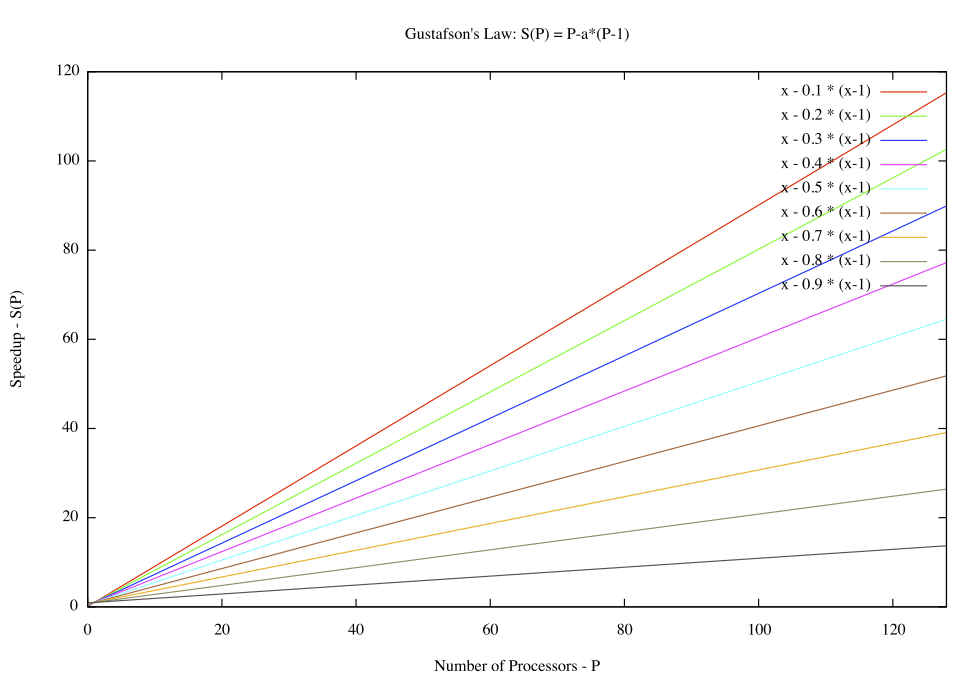
\includegraphics[width=\textwidth]{images/GustafsonsLaw}
	\caption{Gustafson's law states that speedup increases linearly given the 
	amount of 
	work grows evenly with the amount of nodes available to process it. (Image 
	source: 
	Wikimedia Commons~\cite{gustafsonslawimage})}
	\label{fig:gustafsonsLaw}
\end{figure}


%Scalability models

\section{Scalability in cloud infrastructures}
\label{sec:cloudscalability}

Public infrastructure clouds (IaaS clouds) make computing resources available to
customers on a pay per use basis. Customers provision virtual servers, storage
and networks from a pool of physical resources. Part of the allure of IaaS
clouds is that the availability of further resources is made to seem infinite.
Cloud service providers do set limits to the size of deployment under a single
account, but those limits can be raised by separate agreement. The initial
limits are there more to avert denial of service attacks than to safeguard
against actual resource depletion.

It is apparent that clouds are massively scalable systems in terms of
performance, reliability, cost, maintenance and a multitude of other quality
attributes when the size of deployment of physical hardware on which the virtual
resources are provisioned varies. Cloud computing takes distributed computing
forward by increasing dynamism in the structure of distributed systems.
Virtualization enables quick provisioning and deprovisioning of servers, storage
and networks. Setting up a public cloud infrastructure for a new business can be
accomplished in a matter of minutes or hours. The pay-per-use model enables
quick responsiveness to change since adding servers to the environment does not
come with a large up front cost. Similarly, when removing servers from the
system, the released capacity will not necessarily go to waste. It becomes
available to other users of the cloud.

This thesis focuses on the user level of IaaS clouds and the benefits attainable
at that level for building scalable information systems. The underlying physical
implementation of a cloud and scalability therein is left mostly out of scope.
Higher levels of the cloud service stack (PaaS, SaaS) are not discussed
directly, but the elasticity measures presented in later chapters do apply to
them as well.

In cloud context, the basic principles of scalability remain as discussed in
chapter \ref{sec:scalability}. Vertical scaling is achieved by adjusting the
performance of existing virtual machines by changing the amount of available
resources. This can imply relocating the virtual machine to a different physical
host if the current host can’t accommodate the scaled up
VM~\cite{Verma2010-CostOfReconfigurationInCloud}. In practice, vertical scaling
is currently slower than it could be due to limitations on adjusting CPU and RAM
dynamically at runtime~\cite{VRB11}. Changing these parameters requires a
restart and, for example on Amazon EC2, a newly provisioned VM instance will
replace the old one. The process is heavy considering the gained benefit and as
discussed above will grow exponentially expensive when resource demands
increase.

Horizontal scaling is where clouds excel. Virtual machines are cloned as needed
and load is balanced among them. Scaling the network, load balancers and other
infrastructure tools like monitoring is needed when the system grows to surpass
their capacity~\cite{VRB11}.

\subsection{Rapid elasticity}

A cloud is said to be elastic~\cite{nistdefinition} if the resources it provides
can be provisioned and deprovisioned dynamically and automatically. This implies
the necessity to monitor the cloud so that provisioning decisions can be made
based on performance data. Provisioning must be automatic, i.e. decisions to
scale out or scale in should be acted on without human intervention. This
implies the need for cloud customers to access a programmatic interface with
which cloud provisioning actions are carried out. The actions should resolve as
fast as possible to enable constant matching of the size of deployment to
service demand.

The benefit of elasticity is realized when the gap between demand and capacity
can be kept as small as possible (see figure~\ref{fig:oldVsNewScalability}). When
demand increases and more capacity is needed, rapid elasticity can enable the
service to scale out quickly enough so that no requests need to be refused.
Scaling in rapidly when demand decreases means unneeded resources are kept
reserved for a shorter time and consequently less money is wasted on unused
capacity. The utilization rate of provisioned resources can be kept at a better
level compared to a system that would prepare for demand spikes by
overprovisioning resources which then end up being idle during non peak demand.

\begin{figure}[h!]
	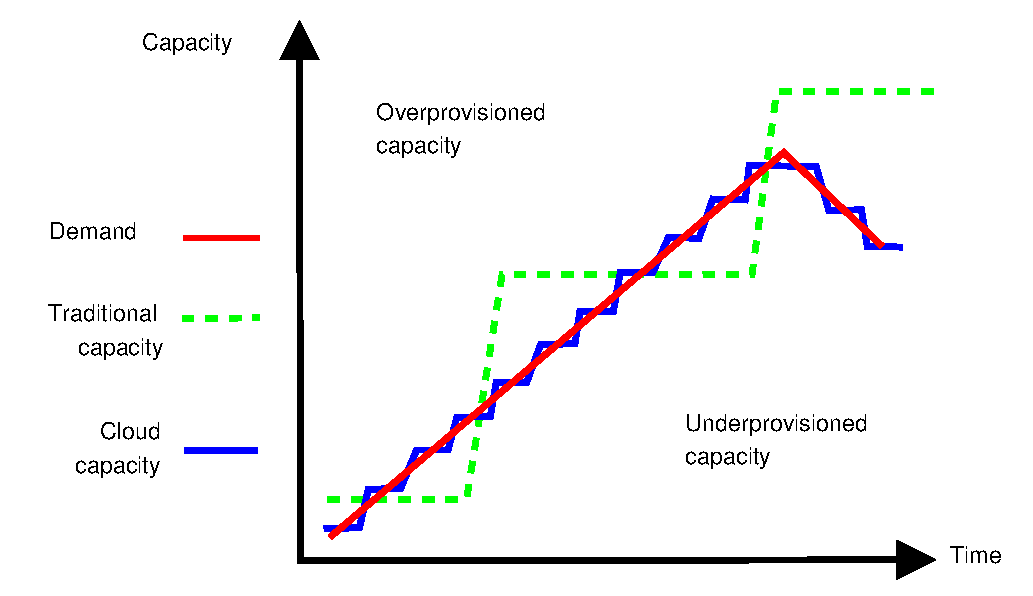
\includegraphics[width=\textwidth]{images/oldVsNewScaling}
	\caption{Elastic scaling allows capacity to closely follow demand whereas
	traditional non-virtualized capacity is slower to provision and typically
	remains unused but reserved when demand decreases.}
	\label{fig:oldVsNewScalability}
\end{figure}

\subsection{Virtual machine lifecycle} \label{sec:VMLifeCycle}

Rapid elasticity is all about adjusting the size of a system by instantiating
new virtual machines (VMs) and terminating existing ones. This takes the VMs
through a lifecycle. Optimizing this lifecycle is key to successful rapid
elasticity.

The VMs go through a number of phases during the lifecycle. The high level
phases from an application perspective are

\begin{itemize}
\item template preparation,
\item instance configuration,
\item instance start,
\item instance contextualization,
\item instance monitoring (running state) and 
\item instance termination.
\end{itemize}

In the template preparation phase, the virtual machine and its data is prepared
up to a point from which it can be instantiated in the cloud. The template could
be a basic installation of an operating system on virtual hardware or further
specialized for a specific purpose. The tradeoff between generic and specialized
templates is the time it takes to configure and contextualize an instantiated
generic VM for a specific purpose and, on the other hand, the
effort needed to maintain specialized templates which can be applied quickly to
newly provisioned VMs.

Instance configuration is the first phase on the way to instantiating a specific
VM instance from the template. This phase may include steps like choosing the
size of the VM instance i.e. how much memory and CPU capacity the instance will
have. Network configuration is set at this phase as well as other virtual
hardware configuration. Security settings such as SSH access keys are configured
in this phase before VM is started up.

With the template chosen and configuration set, the VM instance is ready to be
started. This phase is in the cloud provider’s domain, but customers need to be
able to monitor the progress in order to have up to date information on their
deployment. Behind the scenes, the cloud provider chooses a physical server on
which to allocate the VM instance and makes the necessary changes in their
system to allocate portions of physical CPU, memory, storage and other resources
to the VM.

When the start is done, the customer system will learn of the availability of
the new instance via some reporting mechanism offered by the cloud provider.
This is typically an API query over HTTP, i.e. a request-response cycle. An
event mechanism whereby the cloud notifies the customer would be preferred to
shorten feedback time or the need to busy loop querying the status, but
scalability and security considerations on the cloud provider side may prevent
such a scenario.

After starting up, the virtual machine needs to be contextualized for the
dynamic runtime environment of the service it is part of. The VM could be added
to a group of workers fetching work items from a queue or added to a load
balanced cluster of application servers, for example. Monitoring and other
infrastructure services are configured with runtime information at this point.
To work around waiting time in a scenario where a controller component would
connect to the new VM to perform contextualization tasks after it starts up, the
virtual machine may be configured to pull its context from another server by
executing a script at startup. Context may additionally be provided as a
mountable block storage volume separate from the template. The Open
Virtualization Format (OVF) standard advocates the use of ISO CD images for this
purpose~\cite{ovf11}. Amazon and Eucalyptus among others provide a local network
service for querying instance specific metadata over HTTP.

There has been a lot of research activity regarding the contextualization phase
in the form of describing one-off solutions to accomplish a specific goal like
joining instantiated VMs to a scientific computing
cluster~\cite{Kijsiponge2010}, standardizing an interface between VM instances
and a configurator component to separate concerns of the VM internal
implementation and deployment configuration by the inversion of control
principle \cite{Liu2011} and using this phase to carry out tasks related to a
higher level service management approach ~\cite{frominfratoservice}
\cite{Kirschnick2010} \cite{Chapman2010}.

After contextualization, the VM instance is in the running state. The VM carries
out its tasks and reports its status as configured until, at some point in time,
the VM will be shut down. The termination phase is where the VM should inform
all related system components of its eventual termination so that the system as
a whole can react to it by e.g. removing a load balancing setup or monitoring
scope.

These phases need to be customizable so that cloud customers can add their own
logic in them. Template preparation, configuration, contextualization and
termination phases are the main customization points. Automation tools like
Puppet \cite{puppetlabswebsite} and Chef \cite{chefwebsite} exist to help system
administrators carry out configuration tasks. Claudia \cite{frominfratoservice}
proposes a new abstraction layer on top of IaaS to enable more purposeful cloud
service management including use of multiple cloud service providers.

\subsection{Triggers and bounds - monitoring an elastic cloud deployment}

Clouds have the capability to scale, but system specific logic is needed to make
decisions on when and how to scale. Scaling decisions can be based on the
business requirements set for the system. Good requirements are measurable and
unambiguous. What is measurable depends on the monitoring capabilities of the
cloud system. The monitoring subsystem needs to be customizable so that service
specific metrics can be included in the data set and scaling logic. Cloud
providers typically provide monitoring facilities, but separate monitoring tools
like Ganglia \cite{gangliapaper} serve this purpose in hybrid or highly
specialized configurations. With separate solutions, the cloud customer has full
control over the monitoring subsystem and it can be used in private clouds as
well as in hybrid configurations. The tradeoff is having to maintain the monitoring components if they are not provided as a service.

Quality of monitoring data is important to make timely decisions. With large
deployments, the amount of data can be large and analyzing it all can put load
on the system. Data is typically aggregated from service tiers or groups of
servers to reduce the amount of raw data that is to be processed by the
monitoring subsystem. Another way to reduce monitoring load is to gather data at
longer intervals. This quickly reduces the quality of the scaling metrics. Cloud
systems aiming at just-in-time scalability already have to account for
provisioning delays of tens of seconds or a few minutes. If the data on which
scaling decisions are based is also a few minutes old, this makes the total
reaction time sum up to e.g. 10 minutes. Balancing the monitoring overhead and
scaling reaction time is an exercise needed to optimize each system.

The metrics used to make scaling decisions are typically related to performance
or fault tolerance. CPU and network load and available storage capacity are
straightforward metrics on a subsystem level as well as a heartbeat metric
indicating the live status of each VM. System-wide and service specific metrics
like requests handled per second, time spent on each service tier and the size
of work queues are understandable by business stakeholders and therefore usable
for concretely agreeing on and discussing system performance. Such metrics are
typical for quantifying the quality of service (QoS) and are referred to in
service level agreements (SLA) \cite{Boloor2011} with specific that should not be crossed.

%predictive, reactive provisioning, Urgaonkar2008

Operating a system has to be profitable or at least sustainable. Cost is often
the upper bound for scaling a system in the cloud. Business stakeholders need to
set limits above which the system is not allowed to scale based on cost. The
lower bound is set by technical limitations of system architecture or business
requirements on fault-tolerance and availability. Understanding the economics of
IT systems deployed on clouds is a key success factor in the long run
\cite{Suleiman2011}. Cloud adoption in enterprises begun with simple cost saving
goals but is moving towards enablement of lean enterprises capable of quick
changes in business direction~\cite{Marston2011}.

Clouds are a technology which levels the IT system playing field considerably
between startups and large corporations. With the pay-per-use model, large up
front investments in computing infrastructure are not required to start a
business, yet the scalability is available in case the service popularity
explodes.

%quality of elasticity, Suleiman
%performance variation of VMs

% \begin{itemize}
% \item Elasticity: when/how to scale
% 	\begin{itemize}
% 	\item Infrastructure prerequisites
% 	\item Lifecycle
% 	\item Triggers
% 	\item Business considerations
% 		\begin{itemize}
% 		\item Elasticity window (min/max)
% 		\end{itemize}
% 	\end{itemize}
% \end{itemize}


\section{Elasticity}  
\label{sec:elasticity}

This chapter introduces a theory of elasticity based on the concept of a
controlled process loop governed by business requirements. Metrics are
identified as tools for defining rules that govern a system's measures to stay
conformant to the requirements. The concept of \textit{utility} of a system's
performance based on multi-criteria analysis of conflicting requirements is
developed. The overall utility over a range of time is introduced as
\textit{quality of elasticity, QoE} and the ability of a system to maximize its
utility within a defined range given a specific usage pattern is defined as the
\textit{QoE score}.

The fact that utility and QoE are based on business requirements is key here. Cloud adoption in enterprises is increasingly a step towards making the business more agile instead of saving on IT operations costs~\cite{cloudberkeleyviewacm}. The QoE concept facilitates measurement and scoring of system behavior given a set of business requirements. The system's performance can be optimized by varying either the cloud platform, the way the elastic scaling is handled or the parallelizability of the application implementation. The direction and need for optimizations originates from the business requirements and the QoE results are understandable by business stakeholders. This enables a quick feedback loop between business and IT stakeholders.

\subsection{Elasticity as a controlled process}
\label{sec:elasticity_as_a_controlled_process}

Efficient cloud deployed applications can change their deployment configuration in a matter of minutes if not seconds. To effectively manage a system at such speeds it
is essential that reactions to regularly occurring or anticipated events are
built in to the system and automated.

Concepts from process control theory and autonomic computing can be applied to
implement a cloud application system which knows its state and reacts to changes
in it. An essential part of such a system is a controller component external to
the application itself. The responsibilities of such an \emph{elasticity controller}
are to monitor the system, analyze the metrics, plan corrective actions and
execute them. This is known as a MAPE-K control
loop~\cite{Huebscher2008}\cite{Mueller2009} named after its phases (Monitoring,
Analysis, Planning, Execution, Knowledge). The knowledge in MAPE-K loops is
shared data between the actual MAPE phases. The loop is illustrated in figure~\ref{fig:mape-k}.

The cloud application deployment is monitored and the configuration is adjusted
based on metrics reported by monitoring agents (software components) attached to
the application or its environment. This attachment can be non-intrusive, where
the agent is located outside the application and monitors external phenomena
like network traffic or CPU load. Intrusive monitor attachment works by
instrumenting the execution environment or application itself for monitoring.
For example, a Java virtual machine (JVM) can be instrumented using the
java.lang.instrument API to monitor the internal workings of the JVM. Aspect
oriented programming can be used to instrument at the application level to
monitor metrics unique to the application or its business logic.

\begin{figure}[h!]
	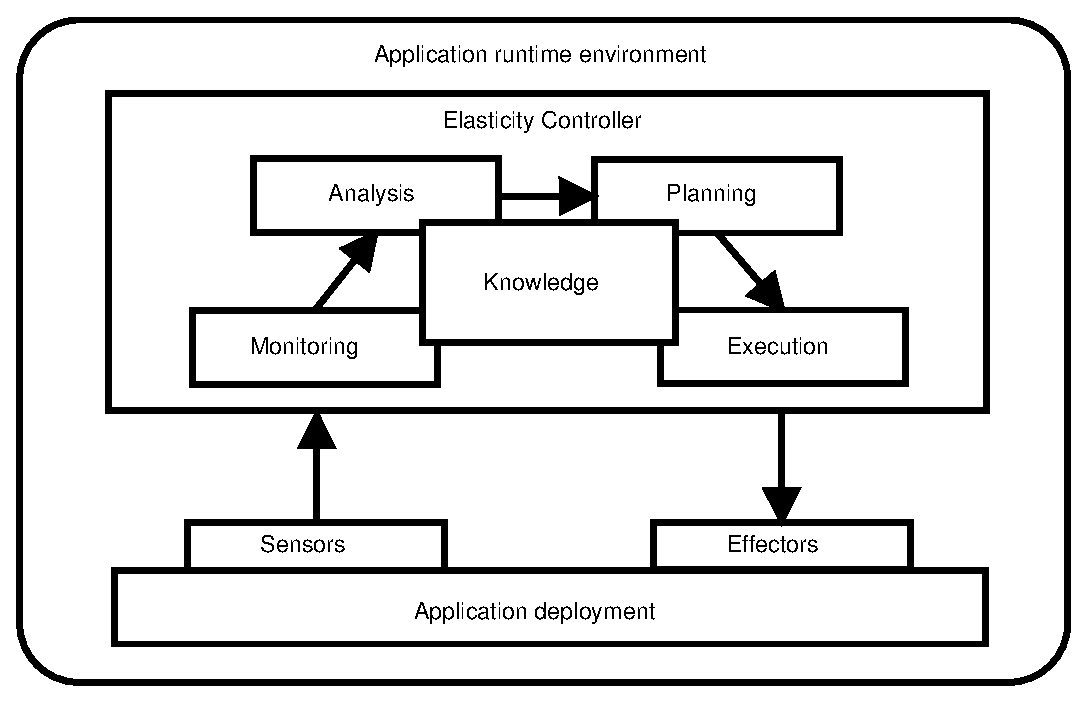
\includegraphics[width=\textwidth]{images/mape-k}
	\caption{The elasticity controller's functionality is modeled after the \mbox{
	MAPE-K} control loop.}
	\label{fig:mape-k}
\end{figure}

Monitoring data is analyzed by the controller in the corresponding phase of the
MAPE-K loop. The raw sensor data is turned into knowledge in this phase. The
MAPE-K knowledge can be an advanced modeled abstraction of the system where the
data is fed into or simply a group of variables reflecting the state of the
monitored system now and the way it is changing over time.

Analysis of the system model may indicate that one or more criteria of
acceptable system behavior are no longer met (reactive trigger) or some metric
is about to exit its tolerated range (proactive trigger). Given such a
situation, the controller will enter the planning phase with the purpose of creating
a plan of action to bring the metric values back to or keep them in the
tolerance zone. This plan can be based on a set of rules that govern the
operation of the controller component or again a more elaborate model driven
approach which approximates the behavior of the actual system.

The execution phase is where the controller or its delegate effector components
interface with the application and the cloud environment to carry out the actions
decided in the planning phase. This phase relies on automation APIs available
for the environment and the runtime configurability of the application.

The executed actions will cause changes in the behavior of the system which are
then reported back to the controller in subsequent control loops.

\subsection{Rules to satisfy requirements} The control loop needs metrics that
are relevant to the system in question and bounds to specify acceptable value
ranges for the metrics. Each metric and its acceptable range represent a
\emph{requirement} for the controller. Rules for controlling the system are
created with the purpose of making sure the system will always meet these
requirements.

Requirements expressed in terms of the implementation technology (system load,
network traffic, etc.) are straightforward to set up for monitoring and further
processing. If non-technical stakeholders like business decision makers are
involved in the requirements elicitation, technical requirements may be
difficult to communicate understandably. Therefore higher level requirements
(e.g. cost per visit to a website, type of user activity, etc.) expressed in
business terms may be the starting point of defining the elasticity requirements
for a system.

To monitor and make scaling decisions based on metrics expressed in business
terms, it is necessary to instrument the application code or monitor the state
of the application's domain model (database). This kind of monitoring takes more
effort compared to non-intrusive technical metrics since the monitoring has to
be customized for the application. The choice of customization or relying on
lower level metrics is a tradeoff one has to make when designing an elastic
system. A mapping from business requirements to technical requirements~
\cite{Chen2008}\cite{Emeakaroha2010}\cite{Wu2011}\cite{Suleiman2011} may be
necessary to facilitate communication of the requirements from their source down
to the implementation of the controller.

\subsection{Multi-criteria decision analysis} Often the requirements given for
the performance of a system conflict each other. If, for example, a system is
optimized in terms of response time by adding more virtual machines to the
deployment, cost rises too high to operate the system. Or if memory usage is
minimized by writing data to disk, the performance may suffer due to increased
access time to data. The requirements may form a complex network of this kind of
interdependencies. It quickly becomes difficult to specify simple rules for
satisfying all the requirements simultaneously.

Multi-criteria decision analysis~\cite{Duboc2007}\cite{Ke2012} is a method
for finding an optimal decision considering conflicting criteria. It can be
applied here to formalize the decision making under conflicting requirements.

\missingfigure{Could show conflicting preference function graphs here and a pareto frontier with their mutually optimum points...}

The multiple criteria are considered together by the use of a \emph{utility
function}

\begin{equation}
U(X) = \sum\limits_{i=1}^k w_{i}P_{i}(X) \label{eq:utilityfunction}
\end{equation}

with a normalized range $U(X) \in [0, 1]$ in the domain of real numbers, where a
value of 0 denotes the worst possible utility and 1 denotes that the system
fully satisfies its combined requirements. $X$ is a set of $j$ parameters
$\{x_{1}, \dots, x_{j}\}$ which are needed to calculate the utility. Metric
values and other knowledge of the system state are typical parameters. The
utility function is a weighted sum of $k$ \emph{preference functions} $P_{i}(X)$
with $1 \le i \le k$. Each elasticity related requirement is defined as a
preference function $P_{i}$ with a normalized range $P_{i}(X) \in [0, 1]$, where
a value of 0 denotes the worst possible preference for this requirement and 1
denotes that the requirement has been optimally fulfilled. The weights $w_{i}$
represent the relative importance of each preference function to overall
utility, with $\sum_{i=1}^k w_{i} = 1$.


\subsection{Quality of elasticity} 

The utility function (\ref{eq:utilityfunction}),
given business-related preferences, measures the business utility of a system
with regard to its performance metrics. Plotting the utility over time as the
usage pattern changes shows how the system responds to these changes. A perfectly
elastic system would adjust its capacity to match or slightly surpass the
required level for maximum utility. The aggregate measure of utility over time
shows how well the system responds to changes, i.e. how well the system scales
out and in as a response to changes in its environment.

The \emph{quality of elasticity} (QoE) for a system over time can be quantified
as the integral of the utility function from some moment of time $a$ to time
$b$ divided by the duration of the measurement $b - a$:

\begin{equation}
QoE = \frac{\int\limits_a^b U(X)~dx}{b-a} \label{eq:qoefunction}
\end{equation}

The range for $QoE$ is the same as that of the utility function, i.e. $QoE \in [0, 1]$ in the domain of real numbers. Figure~\ref{fig:utility-qoe} illustrates the QoE concept as the area on a graph between the values of $U(X)$ and the x-axis over time.

\begin{figure}[h!]
	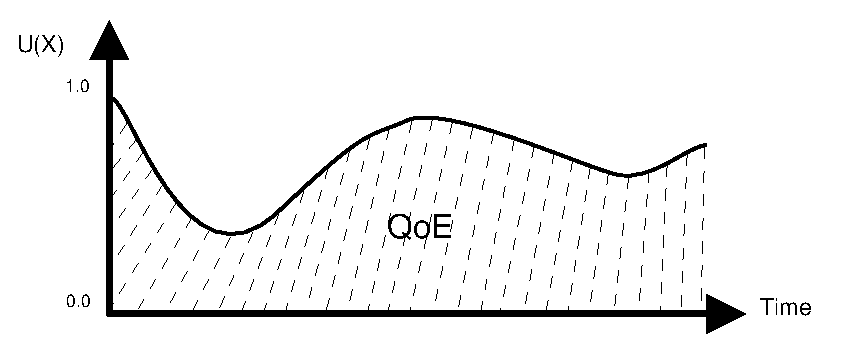
\includegraphics[width=\textwidth]{images/utility-qoe}
	\caption{Quality of elasticity is the integral of the utility function $U(X)$ 
	between two points in time.}
	\label{fig:utility-qoe}
\end{figure}


For real systems the utility function is represented by monitored metric values
gathered over time rather than a mathematical function. In this case the
integral can be approximated by means of numerical analysis. The trapezoid
method \cite{stewart2010calculus} is used for this as the step from each data
point to the next is linear and the method gives exact results in such a case.

The numerical trapezoid method version of the $QoE$ formula is

\begin{equation}
\frac{\int\limits_a^b U(X)~dx}{b-a} \approx 
\frac{\frac{b-a}{2N}\sum\limits_{k=1}^N (U(X_{k-1}) + U(X_{k}))}{b-a} = 
\frac{\frac{h}{2}\sum\limits_{k=1}^N (U(X_{k-1}) + U(X_{k}))}{b-a} 
\label{eq:qoefunctionnumerical}
\end{equation}

where $N$ is the amount of evenly spaced data point intervals and $X_{i}$ with
$i \in [0, N]$ is the set of monitored metric values for utility data
point $i$. The spacing of data points is denoted by $h = \frac{b-a}{N}$ which
solves to $1$ when the data is evenly spaced and available for each interval.
Finally with all simplifications applied, quality of elasticity is calculated
with the following formula:

\begin{equation}
QoE = \frac{\frac{1}{2}\sum\limits_{k=1}^N (U(X_{k-1}) + U(X_{k}))}{b-a} 
\label{eq:qoefunctionnumericalfinal}
\end{equation}

QoE is a measure of the quality of the elasticity controller's decision making
and execution capability in the specific environment it is in. The behavior of
the measured application and the strictness of elasticity related requirements
given for the application influence QoE. The range of possible runtime QoE
values has to be approximated or tested empirically by exercising the system in
order to use QoE as a tool to reason about elastic performance. A threshold
$QoE$ value can be chosen so that whenever below that threshold, the elasticity
controller will work to increase the system's utility. Normalizing the $QoE$
value between this threshold and the maximum 1.0 then gives a score for the
system's elasticity:

\begin{equation}
	QoEScore = \frac{QoE - QoE_{min}}{QoE_{max} - QoE_{min}} 
	\label{eq:qoeScore}
\end{equation}


\subsection{Factors of quality of elasticity}

Quality of elasticity depends on multiple factors which are are both technical
and business related in nature. These factors are discussed in the remainder
of this chapter. Table \ref{table:QoEFactors} on page
\pageref{table:QoEFactors} collects the factors and attributes them to system
components based on the components' infuence on the factor.

For good elasticity, the elasticity controller has to be fed with timely and
correct information on the status of the system. The controller's monitoring
subsystem has to be able to deliver relevant metrics quickly. The data should be
such that it can be reliably used to make scaling decisions. Data jitter can be
a problem as well so often aggregate data is preferred so trends can be
analysed. There is a clear tradeoff between how quickly the metrics show a trend
change and how reliable that indication is. These issues related to
\textit{metric data quality} may need to be tuned specifically for each
application.

With quality metric data, the next step is to react on results of data analysis
quickly and correctly. These factors, namely \textit{speed of decision making}
and \textit{correctness of scaling decisions} are up to the elasticity
controller. Decision making speed can vary based on the the implementation of
the controller. Scaling decisions can be made reactively when metrics pass their
thresholds or predictively based on predictive algorithms. In simple cases the
predictive algorithm could be as simple as specifying time ranges throughout the
day and scaling out or in according to typical usage. Advanced algorithms do
exist for more complicated usage patterns~\cite{Iqbal2011}\cite{Tan2012}\cite{
Roy2011}\cite{Chen2011}\cite{Wilkes2010}\cite{Cunha2011}.
Predictive scaling is possible as long as there is some indicator in the metrics
that can be used to decide that higher load is about to come. For web sites,
sudden spikes of activity like click throughs from a social media discussion
(``Slashdot effect'') with a link to some normally low usage server are
impossible to predict. In such a case, the performance is up to how quickly the
spike of activity is identified and whether the reaction to it matches the size
of the spike.

Scaling out horizontally is helpful if the application is structured to take
advantage of it. The \textit{level of parallelization} exhibited by the
application and its algorithms decides whether the elastic scaling will actually
help with the application's performance. The theory of scalability was discussed
in detail in chapter \ref{sec:scalability}.

Assuming the application is well parallelizable, the \textit{price - performance
ratio} then quantifies the performance received for a certain expenditure
related to scaling out the deployment infrastructure. The ratio is mainly
affected by the cloud provider as it sets the \textit{infrastructure pricing}
for its offering and specifies the kind of resources available. The elasticity
controller and the application implementation also have a role considering the
effective use of the infrastructure. The controller should choose the amount and
type of VM instances to fit the scenario. The elastic application should be
implemented to use infrastructure resources in a way that matches the cloud
provider's capabilities. Advanced optimizations in price - performance ratio may
increase coupling of the application to the infrastructure specifics of the
cloud provider. This can lead to increased effort required if the application is
ever deployed elsewhere, i.e. cloud vendor lock-in.

Further related to price, \textit{billing granularity} affects
QoE~\cite{Brebner2012a}\cite{Islam2012}\cite{Mao2011}\cite{VandenBossche2010}.
The minimum price paid for a provisioned VM instance as well as the billing
interval in the pay-per-use model has an effect on economical use of the
infrastructure. Cost of instantiation or termination could discourage scaling
out and increase the level of commitment to infrastructure. The billing interval
also relates to commitment. The typical hourly billing interval with no extra
cost for instantiation or termination means it is irrelevant whether an instance
is running for a minute or just short of an hour. Effective use of
infrastructure needs to reflect this characteristic of the billing model.

\textit{VM provisioning speed} is a multi-faceted QoE factor. It concerns the
effectiveness of VM lifecycle phases (see chapter \ref{sec:VMLifeCycle}) from
configuration through start and contextualization to termination. An effectively
configured VM image will complete contextualization faster, so the choices made
in the configuration phase affect provisioning speed. If a VM is provisioned
with a baseline configuration of just the operating system, contextualization of
the instance has to include everything from installing application dependencies
to configuring them and announcing the availability of the new instance to the
application infrastructure. Moving some idempotent tasks like software and
operating system update installation from contextualization to configuration can
decrease provisioning time as configuration is done once before and the
configured VM template image is cloned for each VM instance to use. Time spent
in the starting and termination phases is up to the cloud provider as it is the
provider's responsibility to reserve and release physical resources for the
virtual machine. These phases are pure waiting time in terms of the elasticity
controller and the application.

Finally the ultimate bounds for QoE are set by \textit{utility preferences}.
The preferences are modeled above as functions of metric data at a point in
time. The definition of these functions determines the system's utility. The
definitions of these functions need to be realistic and applicable to the
deployment environment. If the definitions are unrealistic, the system may not
exhibit any utility or quality of elasticity as defined here. The preferences
may need to be defined together with technical and business stakeholders to
arrive at workable results. Preferences typically consider cost, response
time, throughput and usage of storage space, memory or other resources but
could be anything that is measurable and for which measured trends can be
mapped to elastic scaling operations. An elicitation method like the
Architectural Tradeoff Analysis Method~\cite{ATAM} can be used to elicit the
preferences from stakeholders. The ATAM method finds quality attributes that
are pivotal to the success of a system to its stakeholders, but appears to
require a lot of effort if applied to its full extent. Research on eliciting
scalability preferences in particular also exists~\cite{DubocUtility}.

%\clearpage
	\begin{table}[h]
\resizebox{\linewidth}{!}{
	    \begin{tabular}{| m{6cm} || >{\centering\arraybackslash}p{2cm} | >{\centering\arraybackslash}p{2cm} | >{\centering\arraybackslash}p{2cm} | >{\centering\arraybackslash}p{2cm} |}
	    \hline
	    \multirow{2}{*}{\textbf{QoE Factor}} & \multicolumn{4}{c |}{\textbf{System Component}} \\
	    & Elasticity Controller & Cloud Provider & Application & Business modeling \\ \hline

		Price - performance ratio & X & X & X & \\ \hline
		Infrastructure pricing & & X & & \\ \hline	    
		Billing granularity & & X & & \\ \hline
	    VM provisioning speed & X & X & X & \\ \hline
	    Metric data quality & X & X & & \\ \hline
	    Decision making speed & X & & & \\ \hline
	    Correctness of scaling decisions & X & & & \\ \hline
		Level of parallelization & & & X & \\ \hline
		Utility preferences & & & & X \\ \hline
	    \end{tabular}
}
	    \caption{QoE factors and the system components which can affect them.}
	    \label{table:QoEFactors}

	\end{table}
% \subsection{Elasticity controller architecture}

% Technology independent explanation of elasticity controller architecture goes here.\todo{Is tech independent controller architecture really still todo or can it be skipped?}

% %controller related architecture items
% \begin{itemize}
% \item elasticity enables design for failure
% \item The role of the controller component
% \item layers in cloud reference model (Tung2011) SYMPOSIUM PAPER, maybe Kirschnick2010 instead? Also CEM11, Kranas2012
% \item Interfaces
% 	\begin{itemize}
% 	\item Application insight (sensors)
% 	\item Cloud infrastructure (actuators)
% 	\item Management information systems (reporting)
% 	\end{itemize}
% \item Scaling algorithms/rules based on metrics \& quality attributes
% \item elastic service definition language (Chapman)
% \item Claudia tool
% \end{itemize}

\subsection{Elastic application architecture}
\label{sec:elasticApplicationArchitecture}

Successful deployment of applications and services on a cloud infrastructure
requires a scalable application architecture. The cloud is not a silver bullet
for scalable software. The software has to be built to take advantage of the
environment.

Algorithms for parallel computation like MapReduce and architectural patterns
like master/worker and cell based architecture \todo{citation of master/worker and cell based architecture patterns} are important building blocks of
harnessing the processing power of a cloud service. The general rule is to
design the architecture so as to have as few as possible shared components in a
deployment. Shared components will end up being the bottlenecks or hotspots when
scaling out for two reasons; They get hit the hardest from multiple other system
components when the system is under heavy load and they are often harder to
scale themselves~\cite{caseforsharednothing}. Unavailability of a
shared component can have far reaching effects on the whole application. Shared
components are actually single points of failure~\cite{cloudarchitecturepatternsbook}.

Public cloud services are built on commodity hardware. The durability and
serviceability of this kind of hardware is by no means in the same class as that
of mainframe hardware. The way to cope with failure of relatively cheap hardware
is to accept it happens and design for
failure~\cite{cloudarchitecturepatternsbook}. Cloud resource pricing is based on
low margins and high volume and best practices advocate ``buying insurance'' by
adding redundancy at every step~\cite{Varia2010}.

Designing for failure implies automating infrastructure and application
deployment and maintenance tasks as fully as possible. Automated recovery from
server failures can be implemented quite simply by terminating a misbehaving
server instance and provisioning another one to replace it. This is in fact one
of the scenarios Amazon Web Services covers in their SLA~\cite{ec2sla}. Notable
omissions from the SLA are server instance uptime and performance. This
underlines the design for failure philosophy of their cloud service offering.

Notable cloud applications apply this principle by making it standard practice
to simulate failures in the infrastructure. The streaming movie service Netflix,
for example, has built and open sourced a component of their infrastructure
called Chaos Monkey which randomly shuts down virtual machine instances in their
production environment. The existence of such a service focuses developers to
design fault tolerant solutions. Research on this kind of failure injection
frameworks has lead to e.g. the idea of a generic failure generation
service~\cite{FAASBerkeleyTechRep} which could be a standard part of a cloud
provider's services.

Knowledge of failures is key to the design for failure approach. Monitoring the
application and the infrastructure is therefore an important architectural
aspect. Cloud providers offer monitoring services that focus on the
infrastructure performance, but application specific monitoring has to be set up
in order to be able to handle failures from a business requirement and service
level agreement perspective as well as technically. An additional benefit of not
relying on the cloud provider's monitoring is avoiding cloud vendor 
lock-in~\cite{Petcu2012}. With external services like the open source Ganglia
monitoring system~\cite{gangliapaper} or commercial alternatives like New Relic
or AppDynamics, it remains possible to add redundancy to the architecture also
at the cloud provider level by deploying on more than one cloud.

Feeding the monitoring system with metrics from the application is a kind of a
glorified logging task. Aspect oriented programming can be used to inject
metrics to business logic without adding complexity. Manually written wrapper
classes with metrics instrumentation are another albeit more disruptive
approach.

%app related architecture items
% \begin{itemize}
% \item elasticity enables design for failure
% 	\begin{itemize}
% 	\item Quality of elasticity
% 	\item Scaling metrics
% 		\begin{itemize}
% 		\item Requests per time period?
% 		\item Depth of work queue?
% 		\item Computational patterns?
% 		\item Event broadcast mechanism?
% 		\item Other way to relay information?
% 		\item Aspect oriented? Cross-cutting concern
% 		\item Latency
% 		\item Costs (VM hours, ...)
% 		\item SLA
% 		\end{itemize}
% 	\end{itemize}
% \end{itemize}

% ARCHITECTURE STUFF:

% Parallel computation needs to have architecture level facilities.

% Web applications are easy in this respect as long as the database does not form a bottleneck. That can be mitigated by relaxing ACID to BASE, for example.

% MapReduce is another type of algorithm that is straightforward to implement
% architecturally. Split computation into tasks, send them away to the cloud and
% combine results when you get them back.

% Statelessness is an important property for scalable architectures. The components involved in scaling should not contain state information.

% Anything that intrinsically requires serial computation is bad and can't be
% helped with architectural excellency.

% Master/Worker pattern description here. 

% Cell based architecture? http://highscalability.com/blog/2012/5/9/cell-
% architectures.html

% IEEEXplore: cloud application architecture

% High availability archicture, divide functionality in zones horizontally:
% http://www.oracle.com/technetwork/articles/cloudcomp/jimerson-ha-arch-
% cloud-1669855.html

% Describe difference from machine based vertical silos to a horizontal array of
% independent services.

% Amazon documentation, cloud best practices, architecting for the cloud.

% High availability, high scalability!

%architecture for applications/systems deployed on cloud
%deployment using ovf specification and extensions for elasticity, Galan2009
%---> Not possible in practice so have to roll your own
%SOA is stateless requests, easy to load balance horizontally

%shared nothing architecture.
%cloud reference model layers in context of iaas paas: Tung, 
%
%multitenancy
%
%SPOSAD architectural style
%%avoid vendor lock in
%
%ESOA, ECSA, Tang
%
%Queuing model QoS scaling (PaaS) CRB11
%
%\cite{Tung2011}

\section{Elastic scaling prototype}
\label{sec:elasticScalingPrototype}

This chapter details the elasticity controller prototype that was implemented
for this thesis as a tool to evaluate the controllability of scalable
application deployment on a cloud platform. The aim of the prototype
implementation was to

\begin{itemize}
	\item{find out what solutions exist to implement an elasticity controller
	 without depending on a specific cloud infrastructure provider's elasticity 
	 services,}
	\item{explore the real world problems of making elastic scaling decisions and}
	\item{test the QoE concept in practice.}
\end{itemize}

The prototype was designed to be cloud provider agnostic. The Amazon EC2 service is used here as the deployment platform, but all components are
implemented using open source software with the intention of supporting any
single cloud platform or multiple platforms at once. Deploying an application
over multiple clouds serves to increase fault tolerance. Cloud vendor lock-in can be avoided if an application is not coupled to proprietary APIs supported by a single cloud provider. Vendor lock-in could make migration to other deployment platforms cost-prohibitive in the long run~\cite{Petcu2012}.

The technologies and software components used in the implementation of the
controller as well as the simple controlled application and environment are
presented in the following chapters.

\subsection{Business application}

The ``business application'' used for the tests is a simple Java servlet based
Service Oriented Architecture (SOA) service implemented using the Spring
framework, version 3.1.1. Upon receiving a HTTP POST request, the business
service calculates a million random integers and returns the last one as HTTP
response header. The service is clearly useless for any real purpose and is
simply written to represent a CPU bound highly parallelizable computation task.
The application does not store user state, which makes it easy to spread the
service requests among any number of servers running the same code. The
deployment includes a load balancer node as a single point of entry. Requests
first arrive at the load balancer which allocates them to any number of
configured application servers using a simple round robin algorithm.

The application is deployed on the Amazon Elastic Compute Cloud (EC2) IaaS
platform. All server nodes run the Ubuntu Linux operating system. The minimal
configuration consists of one application server node (jetty) and a load
balancer node (nginx). Further details of system components and their versions
is given in table \ref{table:componentVersions}.

Scaling out for this application means  

\begin{itemize}
	\item{provisioning more application server instances,}
	\item{contextualizing the instances to work as part of the application 
	infrastructure and}
	\item{changing the infrastructure configuration to account for the newly 
	provisioned instances.}
\end{itemize}

Figure~\ref{fig:deploymentDiagram} shows the deployment diagram for the
application along with elasticity controller components which will be discussed
in further chapters.

\begin{figure}[h]
	%\centering
	%\setlength\fboxsep{0pt}
	%\setlength\fboxrule{0.25pt}	
	\centerline{
	%\hspace*{-3cm}
	\rotatebox{90}{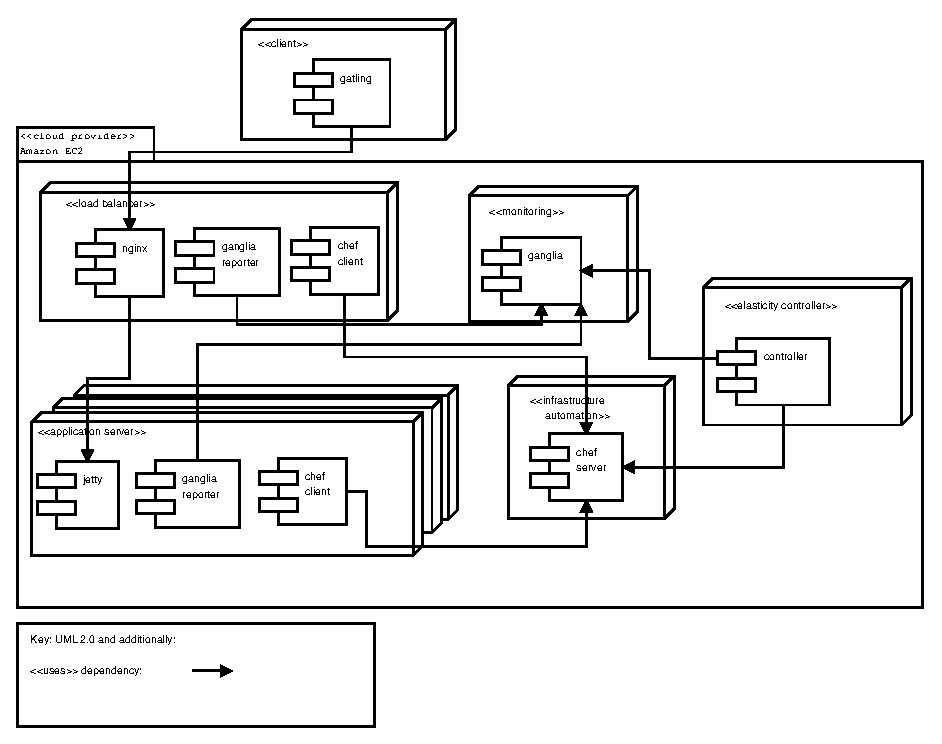
\includegraphics[width=15cm]{images/deploymentDiagram}
	}
	}
	\caption{Prototype deployment diagram.}
	\label{fig:deploymentDiagram}
\end{figure}


The QoE concept needs business requirements to determine the quality of
elasticity. Any requirement can be used as long as it is quantifiable and
measurable in the runtime environment. The requirements for the prototype
application are related to response time and cost. These requirements conflict
as reducing response time by adding more server instances will increase the
cost.

The response time requirement states that the application must respond to
requests within $r_{min} = 0.8$ to $r_{max} = 1.5$
seconds. The response time preference decreases linearly from the maximum value
1.0 down to zero as the response time grows from 0.8 to 1.5 seconds. The metrics used to calculate this preference are response time $r$ and response
time slope $k$. The response time preference function is defined as  

\begin{equation}
P_{r}(r, k) = \begin{cases}
    1, & \text{if $r < r_{min}$}.\\
    0, & \text{if $r > r_{max}$ or $k > k_{spike}$}.\\
    \frac{r - r_{min}}
    	 {r_{max} - r_{min}}, & \text{otherwise}.
  \end{cases}
  \label{eq:responseTimePreference}
\end{equation}

where $k_{spike}$ is a threshold identifying a \textit{spike}, a sudden increase
in requests sent to the system. The spike threshold is defined as $200
\frac{ms}{min}$, i.e. the system is in a spike situation if response time has
increased increased 200 milliseconds per minute. The metric resolution here is 5
minutes.

The slope is defined as 

\begin{equation}
	k = \frac{r - r_{5}}{5}
  \label{eq:responseTimeSlope}
\end{equation}

where $r_{5}$ is the response time 5 minutes prior to the current time.

The response time is measured at the application server using an instrumented
wrapper for the standard jetty request handler class. Network latencies are
therefore unaccounted for.

The cost requirement is specified based on the cost of each service request. As
a simplification, each VM instance is considered to cost 1 currency units per
hour. A maximum cost of 20 currency units is given as the upper bound to limit
scaling out indefinitely. The cost preference function is defined as a
normalized linear mapping in the range $[0,1]$ from a minimum cost per
request $c_{min}$ to a maximum cost per request
$c_{max}$ of 1.0, i.e. 


\begin{equation}
P_{c}(e, v, k, q, t_{vm}) = \begin{cases}
    1, & \text{if $c < c_{min}$ or $v \leq 1$ or $k > 50$ or $q > 0$}.\\
    0, & \text{if $c > c_{max}$ and $v > 1$}.\\
    \frac{c - c_{min}}
    	 {c_{max} - c_{min}}, & \text{otherwise}.
  \end{cases}
  \label{eq:costPreference}
\end{equation}

where $e$, $v$, $k$, $q$ and $t_{vm}$ denote current arrival rate of requests,
amount of application server VM instances currently in use, response time slope,
average queue length at the application servers and maximum average
server throughput (requests per second per VM instance) measured when the average
response time is less than $r_{min}$, respectively. $c_{min}$ is further defined
as the cost per VM instance $c_{vm}$ divided by $t_{vm}$ , i.e.

\begin{equation}
	c_{min} = 
	\frac{c_{vm}}{t_{vm}} 
	\label{eq:costMin}
\end{equation}

where $t_{vm}$ is measured only when $r < r_{min}$.\todo{can the throughput metric be simplified, the response time rule does not make sense? NOT FOR NOW.} 

The application running on \textit{m1.small} instances on Amazon EC2 will
typically handle approximately 3 requests per second with a response time less
than the $r_{min}$ of 0.8 seconds. This makes $c_{min}$
roughly equal to 0.3 currency units.

\subsection{Elasticity controller}

The prototype elasticity controller and its monitoring and infrastructure automation facilities are distributed between multiple server nodes
in the environment as illustrated in figure~\ref{fig:deploymentDiagram}. The controller exists to answer three basic questions on
elastic scaling, namely 
\begin{itemize}
	\item{\textit{when} to scale,}
	\item{\textit{how much} and \textit{in which direction} to scale and}
  	\item{\textit{how} to scale}.
\end{itemize}

These questions map to the MAPE-K phases of analysis, planning and execution.
Here the deployment and execution sequence of the elasticity controller is
described in terms of the MAPE-K control loop (see
figure~\ref{fig:mape-k} on page \pageref{fig:mape-k}).

\textit{Monitoring} is implemented using the Ganglia monitoring
system~\cite{gangliapaper}. The application servers and the load balancer run the
Ganglia monitoring daemon (\texttt{gmond}), which sends metric data to a
separate monitoring server. The Ganglia monitoring server runs both the
\texttt{gmond} and \texttt{gmetad} daemons which together aggregate and store metric
data from all monitored servers. 

The \textit{analysis} and \textit{planning} phases are the responsibility of an
elasticity controller application written specifically for this prototype. The
controller queries the Ganglia server for system state metrics every 20 seconds
and calculates the utility based on the preference functions defined for the
business application. The controller first analyses the system utility. If
utility is below a threshold of 0.7, the controller proceeds to the planning phase.

For the purpose of making a plan to scale the system either out or in, the
controller application uses a \text{scaling function} $S(X)$ to indicate the
needed direction and distance from optimal utility. The range of $S(X)$ is
$[-1\dots1]$. A value of $-1$ represents the maximum impulse to scale in while a
value of $1$ represents the maximum impulse to scale out. To factor in the
direction of scaling, the preference functions are divided into two groups based
on requiring either scaling out or scaling in to improve their value.  The
scaling function then takes the form

\begin{equation}
S(X) = \sum\limits_{i=1}^j w_{i}^{in}P_{i}^{in}(X) + 
		\sum\limits_{i=1}^k w_{i}^{out}P_{i}^{out}(X).
\label{eq:scalingfunction}
\end{equation}

where $P_{i}^{in}$ denotes a preference which requires scaling in and
$P_{i}^{out}$ denotes a preference which requires scaling out to improve. The
weights $w_{i}^{in}$ and $w_{i}^{out}$ are distributed among these two groups so
that $\sum\limits_{i=1}^j w_{i}^{in} = 1$ and $\sum\limits_{i=1}^k w_{i}^{out} =
1$. In practice the prototype used here has one preference ($P_{r}$) for scaling out and one ($P_{c}$) for scaling in, so both their weights are $1.0$.

In addition to the scaling function, the elasticity controller detects trends in
response time by keeping track of the request response time in a 5-minute moving
window. The slope $k_{r}$ of response time is calculated based on the delta of
the metric value 5 minutes ago and currently. If response time has grown more
than 200 ms per minute in the last 5 minutes, i.e. $k_{r} > 200 \frac{ms}{min}$,
the trend is considered a \textit{spike}, a sudden large increase in activity.

With this information, the elasticity controller creates a scaling plan. Scaling
is done in the direction indicated by the scaling function $S(X)$ and the amount
of server instances to add or remove depends on the slope. With gradual growth,
the amount of application server nodes is increased by half. If the response
time slope indicates a spike is underway, the server instance count is
multiplied by three. 

Further thresholds apply to the planning phase. In order to scale out, the
request rate needs to be larger than 2 requests/s. To avoid repeatedly adjusting
the size of the deployment, scaling in requires the scaling utility function
value to be $S(X) < 0.5$.

For scaling in, the amount is decided with the use of the cost preference
function. The cost preference is calculated with decreasing instance count until
it reaches the maximum preference value. Any instances above the count which
yields maximum cost preference are terminated.

With the above definition of the scaling function $S(X)$, it is possible that
positive scale out preferences and negative scale in preferences cancel each
other out or interfere with each other at a time when the metrics clearly indicate scaling is needed in a specific direction. For this reason, the cost preference is considered to be at its maximum in the following situations:

\begin{itemize}
	\item{If the slope is larger than $50 \frac{ms}{min}$. This indicates an increasing load trend.}
	\item{If there are requests queued up at the application server(s), i.e. all available processing threads are processing a request and more requests are waiting to be processed.}
	\item{If there is only one application server.}
\end{itemize}

Similarly the response time function has one special case when it is set to minimum preference. This is when the response time slope indicates a spike. The preference function then indicates the need to scale out regardless of the current response time value.

The controller application delegates \textit{execution} of the plan to an
infrastructure automation tool called Chef. Chef is a cloud age tool which
enables an infrastructure as code approach to IT operations. All installation
and configuration is done with scripts written in Ruby. In Chef terminology,
these are referred to as recipes within cookbooks. Chef manages the state of the
deployment on a separate server which is a part of the infrastructure. Each
server node managed by Chef runs the \texttt{chef-client} daemon which
periodically connects to the Chef server and configures the node to match the
state received from the Chef server.

The MAPE-K \textit{knowledge} is a shared concept between the controller
application, Ganglia and the Chef server. The controller keeps track of trend
averages of metrics it fetches from Ganglia and system contextualization is done
based on system state information managed by Chef. The load balancer server runs
\texttt{chef-client} every 30 seconds. This is how knowledge of application
servers is updated at the load balancer. Similarly the address of the monitoring
server is read from Chef every time a new node is configured (and periodically
during the node's lifetime). Any change in system configuration due to scaling
operations gets updated to live nodes in this way.

Although the monitoring system reports new values every 15 seconds, the moving
average values for metrics take time to reflect a change in system
performance. Response time, for example, is measured as a biased histogram of
1028 data points. The histogram sample uses a forward-decaying algorithm which
favors data from the past 5
minutes~\cite{forwardDecayHistogram}\cite{codahaleHistogram}. Averaged metrics
are used to even out jitter (oscillation) in the measured values that could
trigger unnecessary provisioning operations. The downside is that the metrics
take time to react to significant changes as well. To allow time for the
metrics to react and stabilize after a provisioning operation, the system has
a 3-minute quiet period after each provisioning completes. No new provisioning
operations are started during this time. This gives time for the metrics to
stabilize for a new amount of virtual machines and e.g. data to start actually
arrive from newly provisioned VMs, but also means the system is not responsive
to utility changes during this time. Responsiveness is further hindered by the
time it takes to provision instances, as the total quiet period consists of
first waiting for new instances and then waiting for metrics to stabilize.

	\begin{table}[h]
		\resizebox{\textwidth}{!}{
	    \begin{tabular}{| l | r | p{6cm} |}
	    \hline
	    \multicolumn{3}{| c |}{\textbf{Components in the prototype environment}} \\ \hline
		\textbf{Component} & \textbf{Version} & \textbf{Purpose} \\ \hline
		Jetty & 8.1.7.v20120910 & Web server \& Java servlet container \\ \hline
		Nginx & 1.1.19 & Load balancer \& HTTP server \\ \hline
	    Chef & 10.18.2 & Infrastructure automation tool \\ \hline
	    Gatling & 1.4.1 & Load testing tool \\ \hline
	    Ganglia & 3.4.0 & Monitoring system \\ \hline
		Ganglia Web & 3.5.2 & Monitoring dashboard user interface \\ \hline
		Codahale Metrics & 3.0.0-SNAPSHOT & Java library for collecting 
		metrics from application server and application \\ \hline
	    Ubuntu Linux & 12.04.1 LTS & Operating System on all nodes. \\ \hline
	    \end{tabular}
		}
	    \caption{Server applications and tools used in the prototype.}
	    \label{table:componentVersions}
	\end{table}

\section{Test results}
\label{sec:results}

This chapter discusses the performance of the elasticity controller prototype
and the test application in terms of utility preferences and the overall quality
of elasticity for the application deployment described in chapter~
\ref{sec:elasticScalingPrototype}. Two different testing scenarios are
presented along with results of how the controller responded to the request load
generated by the scenarios. Quality of elasticity is evaluated as a conclusion to the chapter.

\subsection{Test scenarios} \label{sec:testScenarios} 

The elasticity controller was tested under two scenarios. Scenario 1 subjected
the system to a gradually growing rate of requests while scenario 2 generated a
sudden spike of requests. The scenarios were implemented using the Gatling load
testing tool \cite{gatling}.

Gatling simulates users making requests to the application. Each simulated user
sends equal requests, i.e. only one request type is used. The request handler
calculates a million random integers and returns the last one. After receiving a
response, the user waits for a random amount of time between 500 and 800
milliseconds before sending another request. This is repeated for one hour. The
actual time depends on response times and ramp down periods.

The amount of users varies throughout the scenarios. The gradual growth scenario
starts with six users and adds two more every 10 minutes. All users finish after
one hour. The scenario steps with their timings for scenario 1 are:

\begin{itemize}
	\item{\textbf{00:00} - 6 users ramp up in 30 seconds.}
	\item{\textbf{00:10} - 2 users ramp up in 1 second.}
	\item{\textbf{00:20} - 2 users ramp up in 1 second.}
	\item{\textbf{00:30} - 2 users ramp up in 1 second.}
	\item{\textbf{00:40} - 2 users ramp up in 1 second.}
	\item{\textbf{00:50} - 2 users ramp up in 1 second.}
	\item{\textbf{01:00} - 10 users ramp down in 1 second. The first 6 users ramp 
			down in 30 seconds.}	
	\item{\textbf{01:00:30} - Finished ramping down users.}
	\label{gatlingStepsScenario1}
\end{itemize}

The spike scenario starts with three users for five minutes, then gradually adds
six more users during a period of ten minutes and finally starts the spike of 30
users at 00:25. The spike nearly quadruples the user amount during one minute. The
spike lasts for 20 minutes until 00:45. At 00:55 The six user wave starts
ramping down over the next 10 minutes, so that at 01:00, when the first 3 users
ramp down, 3 users from the six user wave are still ramping down. Finally all
users are ramped down at 01:05. The steps with their timings for scenario 2 are:

\begin{itemize}
	\item{\textbf{00:00} - 3 users ramp up in 5 seconds.}
	\item{\textbf{00:05} - 6 users ramp up in 600 seconds.}
	\item{\textbf{00:15} - 6 users fully ramped up.}
	\item{\textbf{00:25} - 30 users ramp up in 60 seconds (spike).}
	\item{\textbf{00:45} - 30 users ramp down in 60 seconds (spike ends).}
	\item{\textbf{00:55} - 6 users ramp down in 600 seconds.}
	\item{\textbf{01:00} - 3 users ramp down in 5 seconds.}
	\item{\textbf{01:05} - Finished ramping down users.}	
	\label{gatlingStepsScenario2}
\end{itemize}

\subsection{Results: Scenario 1}
\label{sec:resultsScenario1}

Scenario 1 exhibiting gradual growth in request rate was handled quite well by
the elasticity controller. Starting off with 1 application server instance and 6
users, a reference throughput ($t_{vm}$ used in cost preference calculation)
rate of $3.4$ requests per second per server was established at 00:07 as show in
figure \ref{fig:referenceThroughputScenario1} on page
\pageref{fig:referenceThroughputScenario1}. Utility (fig.
\ref{fig:utilityScenario1} on page \pageref{fig:utilityScenario1}) stayed above
the scaling trigger value of $0.7$ until the first two users were added at
00:10. The controller took 6 minutes to react to the increased amount of users.
At 00:16, utility fell below $0.7$ due to an increase in response time (fig.
\ref{fig:responseTimeScenario1} on page \pageref{fig:responseTimeScenario1}) to
$1.2 s$ and hence a drop in the corresponding preference function value (fig.
\ref{fig:responseTimePreferenceScenario1} on page
\pageref{fig:responseTimePreferenceScenario1}) to $0.4$. The MAPE-K planning
phase was triggered and concluded with a decision to provision one new VM
instance as scaling utility (fig. \ref{fig:scalingUtilityScenario1} on page
\pageref{fig:scalingUtilityScenario1}) was positive at $0.6$ at the time and
response time slope (fig. \ref{fig:responseTimeSlopeScenario1} on page
\pageref{fig:responseTimeSlopeScenario1}) was under $200$ indicating no spike
was occurring.

Two application server instances were enough to satisfy utility for most of the
test duration. Utility dropped below $0.7$ briefly at 00:21 during the
controller's post provisioning quiet period. This utility fluctuation is caused
by a drop in both response time and cost preference values (fig.
\ref{fig:costPreferenceScenario1} on page
\pageref{fig:costPreferenceScenario1}). The metrics for request rate and
response time fluctuated down and up at this time due to the system adjusting to
the new virtual machine. Averaged metric values are affected immediately when a
new instance shows up in the monitoring system (averaged system wide values are
calculated by dividing a sum of each node's metric value by the number of
nodes). It takes 2-3 minutes after this to start receiving actual correct data
from the new node and for 1-minute and 5-minute averaged metrics to react. The
quiet period accommodates this fluctuation and prevented a hasty further scaling
decision here.

The next significant change in utility was at 00:33. Request rate (fig.
\ref{fig:requestRateScenario1} on page \pageref{fig:requestRateScenario1}) drops
to $2$ requests/s for no apparent reason but then recovers to $3$ at 00:37.
Response time reacts upward to nearly $1.2 s$ a bit later at 00:36 returning to
$0.8 s$ at 00:40. This appears likely to be a slow down in the infrastructure as
the request load did not change at the time. Response time reacts slower than
request rate because it is calculated using a 5-minute median as opposed to a
1-minute mean for the request rate.

At 00:54, utility fell below $0.7$ again. Response time had increased earlier
and starting from 00:50 request rate fell down to $4$ from $6$. This was likely
another infrastructure performance fluctuation as a comparable request rate
change did not happen after 00:40 when 2 more users started making requests
just like at 00:50. On the other hand, the effect of those additional users shows
clearly in response time as it increases to 1 second after the user increase at
00:40. With the response time increase followed by the request rate drop, the
elasticity controller made a further scale out decision to add 1 VM instance.

The added VM arrived late for this scenario. Provisioning started at 00:54 and
continued until 00:59. The metrics show the VM coming properly online just
before the one hour mark at which the Gatling load script terminates. The
completion of VM provisioning is seen in the response time preference value as
it increases quickly at the same time as the VM count metric (fig.
\ref{fig:vmCountScenario1} on page \pageref{fig:vmCountScenario1}) increases.
Then response time preference decreases as the new VM starts reporting response
times and takes time to get up to full speed. The scenario ends at 01:00 and the
1 minute average request rate metric reacts a minute later to drop utility below
$0.7$ again. This triggers another scaling decision whereby 2 virtual machines
are terminated, returning the system to its original configuration of 1
application server instance.

The overall $QoE$ value for this scenario is $0.86$. The system performed
relatively well in terms of quality of elasticity. Normalizing $QoE$ between a
minimum of 0.7 and maximum of 1.0 (eq. \ref{eq:qoeScore} on page
\pageref{eq:qoeScore}) yields a score of 53\% to the system given this
elasticity scenario.

\subsection{Results: Scenario 2}

The second scenario tests the system's behavior under a load which spikes, i.e.
suddenly increases from 9 users to 39 users. Reference throughput used for cost
calculation goes up to $3.6$ this time at 00:12 (fig.
\ref{fig:referenceThroughputScenario2} on page
\pageref{fig:referenceThroughputScenario2}). The difference to the scenario 1 value
of $3.4$ has to be attributed to the cloud infrastructure as the virtual machine
instances are different and hence also the placement on physical hardware at
Amazon's data center is most likely different. The maximum reference throughput
was reached later than in scenario 1 due to the difference in user amounts.
Scenario 2 has 8 users making requests at 00:12 whereas scenario 1 reached its
maximum throughput with 6 users. The VM in scenario 2 could take on more load and still perform as well as the scenario 1 VM. Performance is clearly different
between VM instantiations with the same specifications.

Utility (fig. \ref{fig:utilityScenario2} on page \pageref{fig:utilityScenario2})
was at maximum until the amount of users reached 8. Response time had slowly
increased from 00:08 with the gradual increase of users and lead to utility
dropping below the $0.7$ threshold at 00:16. Provisioning of one VM instance was
started and the VM became operational at 00:20 returning utility above the
threshold. The metrics jittered a lot during the quiet period again as they
adjusted to the new instance. After stabilizing, utility increased back to
maximum at 00:26, just in time to receive the spike.

The spike started at 00:25 with 30 additional users ramping up over the next 60
seconds. The system was clearly not ready to handle this kind of load as the
application server request queues started filling up (fig.
\ref{fig:queueScenario2} on page \pageref{fig:queueScenario2}) which did not
happen at all in scenario 1 (fig. \ref{fig:queueScenario1} on page
\pageref{fig:queueScenario1}). At 00:28 the response time preference (fig.
\ref{fig:responseTimePreferenceScenario2} on page
\pageref{fig:responseTimePreferenceScenario2}) quickly fell from 1.0 to 0.0.
Response time was increasing but the slope metric was close to 0 as response
time now and five minutes prior was nearly at the same level. Utility decreased
below the threshold, but the elasticity controller failed to detect the spike
because of the low slope value. Due to this, provisioning of only one additional
VM instance was started at this time.

The spike continued while the single VM was being provisioned. Its introduction
to the load balancing array understandably did nothing to make this better and
utility was flat at 0.5. Utility did not decrease further because the cost
preference function was at maximum, i.e. the request rate (fig.
\ref{fig:requestRateScenario1} on page \pageref{fig:requestRateScenario1}) was
high enough to keep cost per request low. At 00:34, six minutes after the
misfired single VM provisioning operation, the quiet period ended and the
elasticity controller was able to add more VM instances. This time 9 more were
added, as the controller is configured to triple the amount of VMs if it detects
a spike.

One of the 9 VMs failed in the contextualization phase and at 00:40, 8 new
application server instances started receiving requests. During the quiet period
and even after it until 00:44, utility was below the 0.7 threshold, but no
scaling operations were executed. The scaling utility metric (fig.
\ref{fig:scalingUtilityScenario1} on page
\pageref{fig:scalingUtilityScenario1}), which indicates whether to add or remove
instances, was negative but not below 0.5, so scaling was not executed. Both the
response time and cost preferences were below 0.8 at this time and they canceled
each other out in the calculation of scaling utility. The metric stabilization
took longer than previously due to the large amount of 8 new VMs, so the post
scaling quiet period failed to protect the system. However as the metrics
influence scaling utility in opposite directions, a further scaling operation
was avoided here right before the spike ended.

The spike ended gradually between 00:45:00 and 00:45:30. The request rate
metric began to show this at 00:46. Cost preference decreased and response time
preference increased to maximum. The cost increase triggered removal of 8 VMs at
00:46:30. The termination caused a sudden drop in request rate which brought
utility down to 0.5 due to rising cost per request per server. This was during
the quiet period, however, and the metrics stabilized prior to the end of the
period.

With the spike over and 3 VM instances left, the system ran at approximately
0.85 utility until 00:55. After this the 6 user ``second wave'' started ramping
down over the next 10 minutes. Utility slowly decreased due to this until a
bigger impulse was given by the ramp down of the 3-user ``first wave'' at 01:00.
Metrics reacted to this at 01:00:30 and the controller brought the system down
to its initial configuration of 1 application server instance. The remaining
second wave users finished their rampdown at 01:05 with utility already back at
maximum since 01:02:30.

The overall $QoE$ value for this scenario is $0.78$. The system did not perform
well with regard to the spike usage profile represented by this scenario. The
scaling threshold was set at $0.7$. Normalizing $QoE$ between a minimum of 0.7
and maximum of 1.0 (eq. \ref{eq:qoeScore} on page \pageref{eq:qoeScore}) yields
a score of 27\% to the system given this elasticity scenario.

\subsection{Notes on quality of elasticity}

The QoE scores obtained in the tests were 53\% for scenario 1 and 27\% for
scenario 2. The controller is better at managing elasticity when the metrics
change slowly like in scenario 1. Main reasons for this are the delays observed
after a scaling decision execution was started. It took roughly 3-4 minutes from
decision to the point where a new virtual machine was available to service
requests and another 3 minutes for the quiet period during which metrics were
allowed to stabilize for the new configuration. The elasticity controller
prototype took a simple approach to running the MAPE-K loop; it was run
sequentially, one at a time. the total time between two control loop executions
could range from 20 seconds (no scaling decisions made) to 6-7 minutes when the
scaling plan execution phase waits to receive control of new VM instances and
contextualizes them. An improvement could be to run the control loop during
provisioning and the quiet period and implement the possibility to cancel an
operation if the metrics start to give an opposite indication while provisioning
is in progress.

The metrics, which are polled every 15 seconds, are averaged for stability which
makes the slower to react to changes. A 5-minute average for response time was
used as it was readily available in the Coda Hale Metrics open source project,
but a faster metric could have helped with the reaction time and allowed a
shorter quiet period for the control loop. Similarly the response time slope
metric was calculated over 5 minutes, which worked against spike detection in
scenario 2.

The cost metric is rather superficial in these tests as the size of the
deployment is small and hence small changes in user amount are percentually
large. In real systems where this kind of calculation becomes relevant, there
would be a business case for the system and a reasonable cost preference could be
derived from it~\cite{Suleiman2011}. Issues like billing period granularity,
which this prototype does not consider, then rise to a more important status.
The controller would then have to keep track of billing cycles and other real
time cost factors to properly optimize QoE in terms of cost.

The cloud infrastructure itself played a variable role in the $QoE$ results.
Particularly in scenario 1, the request rate dropped twice for no apparent
reason caused by the scenario. As the effect of this was to only reduce utility
within the threshold limit, these performance fluctuations reduced $QoE$ with no
reaction from the elasticity controller. In scenario 2, one of the total 15 VM
instance provisioning operations failed. This is notable because the operations
are automated and hence user error is eliminated as a possible cause. Many
things can still fail on many levels, as Amazon runs the EC2 service on
commodity hardware and the infrastructure is accessed over the Internet and
provisioning relies on the availability of many other Internet services like the
Ubuntu package repositories. 

As the cloud provider business model is based on guarantees of quantity over
absolute guarantees of quality, the design for failure approach~\cite{Varia2010}
can be used to mitigate this kind of risk. Given the pay per use pricing model,
it is inexpensive to overprovision by a certain percentage as an insurance
against failed VM delivery or performance fluctuations.

The controller logic implemented for the prototype is based on a reactive
concept. The controller analyses historical data and makes decisions based on
that. Introducing a predictive analysis model could help maximize $QoE$
~\cite{cloudberkeleyviewacm} as the controller could know to prepare for future
load before it arrives by either provisioning new resources or deciding not to
terminate old ones just before load is about to increase. In straightforward cases
a simple schedule based analysis could help as e.g. web applications typically
have usage profiles peaking when people work or are awake and periods of
inactivity outside of business ours or during the night.

\section{Conclusion}
\label{sec:conclusion}

This thesis presented an overview of cloud computing service levels and focused
on elasticity at the IaaS level. Theory of scalability was examined and divided
it into horizontal, vertical and structural (algorithmic) dimensions. Tradeoffs
arising from designing applications for scalability were identified as
difficulty of synchronizing state, use of unscalable shared resources which
quickly become bottlenecks, exponential cost of vertical scaling and design
effort for structural scalability.

The theory of horizontal scaling was examined further as that is the kind of
scaling most applicable to cloud applications. The limits of scalability were
discussed based on Amhdal's~law \cite{amdahlslaw} and Gustafson's
law~\cite{gustafsonslaw} in chapter~\ref{sec:scalabilityBounds}. Analysis of
scalability based on multi criteria analysis of metrics was presented based on
the work of Duboc~\cite{Duboc2007}.

The scalability theory was taken into cloud infrastructure context in
chapter~\ref{sec:cloudscalability}. The concept of rapid elasticity was
introduced and the lifecycle of an elastic virtual machine instance was
walked through. Availability of data on the system's performance and the quality of
that data was identified as a key success factor for cloud scalability.

Cloud platform and application elasticity was examined further from the
viewpoint of a MAPE-K control loop in chapter~\ref{sec:elasticity}. The concept
of utility of an application deployment was developed based on multi-criteria
analysis of business requirements. Quality of Elasticity (QoE) was introduced as
a metric of utility over time. To facilitate comparisons and contextualization
of QoE to a specific system in a specific environment, a QoE score metric was
defined as the normalized value of QoE between a deployment specific lower bound
threshold and maximum.

Design principles of elastic application architectures were discussed briefly in
chapter~\ref{sec:elasticApplicationArchitecture}. The design for failure
philosophy is a key point in thinking of the fitness for purpose of cloud
provider SLAs. The cloud provider business model and offering is fundamentally
different from the traditional IT operations without virtualization. Designing
applications so that they can handle infrastructure failures is key to success.

A prototype elasticity controller implementation  is presented in
chapter~\ref{sec:elasticScalingPrototype}. The prototype is then put to test in
chapter~\ref{sec:results}. The results confirm the applicability of the
controller to its purpose and indicate areas in need of further study that have
the potential to improve the QoE scores attained with the controller. In
particular the quality and reactiveness of metrics, VM provisioning speed and
parallelization of the elasticity controller's decision making functionality are
identified as areas of possible improvement. The quality of the controller's
decisions could be improved by moving from a reactive analysis model to a
predictive one.

The QoE results correctly indicate that the elasticity controller handled test
scenario 1 better than scenario 2 in terms of the business requirements used
to define QoE for the prototype. The QoE concept should be put to further test
using varying business requirement definitions to determine its universal
applicability to measuring cloud elasticity.

\clearpage
\appendix

\section{Figures for test scenario 1}

\begin{figure}[htbp]
	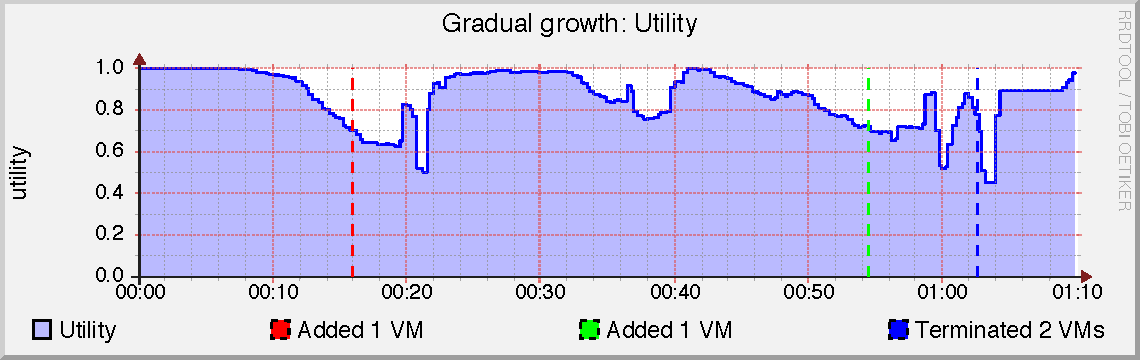
\includegraphics[width=\textwidth]{images/utilitygraph-test21}
	\caption{Utility during test scenario 1}
	\label{fig:utilityScenario1}
\end{figure}

\begin{figure}[htbp]
	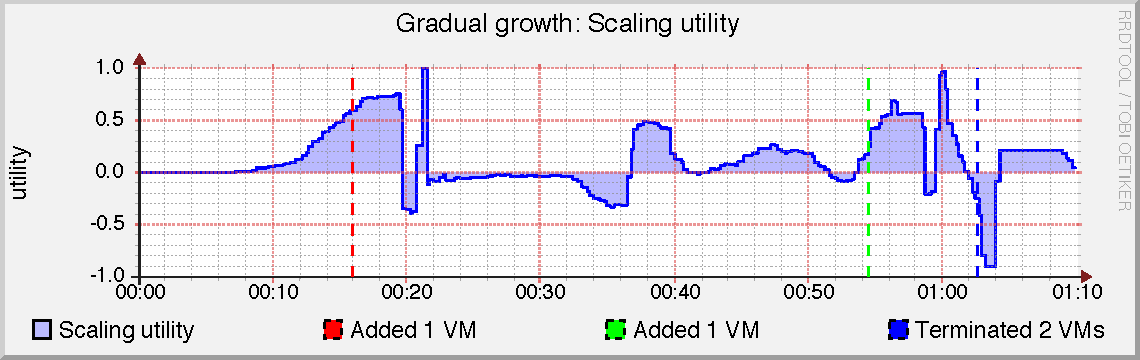
\includegraphics[width=\textwidth]{images/scalingutilitygraph-test21}
	\caption{Scaling utility during test scenario 1}
	\label{fig:scalingUtilityScenario1}
\end{figure}

\begin{figure}[htbp]
	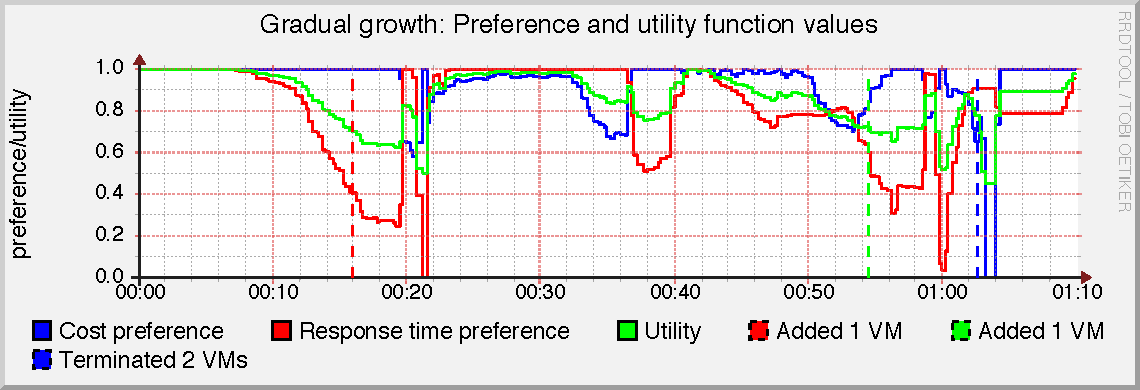
\includegraphics[width=\textwidth]{images/preferencesgraph-test21}
	\caption{Combined preference function and utility values during test scenario 1}
	\label{fig:preferencesScenario1}
\end{figure}

\begin{figure}[htbp]
	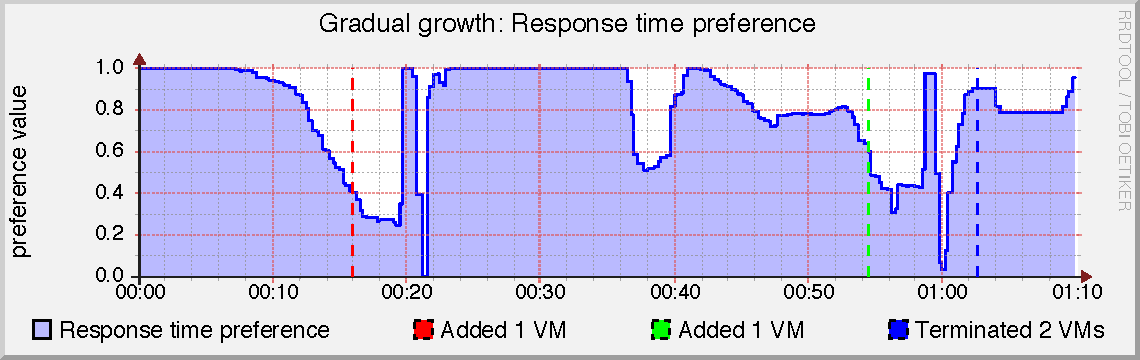
\includegraphics[width=\textwidth]{images/responsetimepreferencegraph-test21}
	\caption{Response time preference function values during test scenario 1}
	\label{fig:responseTimePreferenceScenario1}
\end{figure}

\begin{figure}[htbp]
	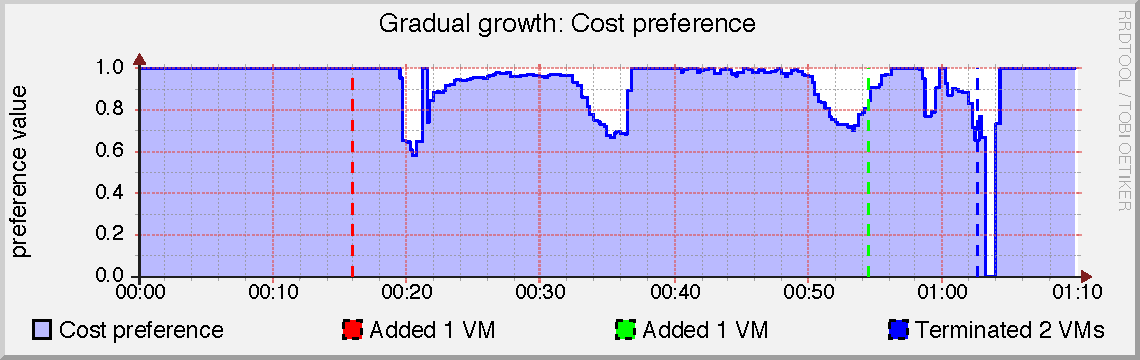
\includegraphics[width=\textwidth]{images/costpreferencegraph-test21}
	\caption{Cost preference function values during test scenario 1}
	\label{fig:costPreferenceScenario1}
\end{figure}

\begin{figure}[htbp]
	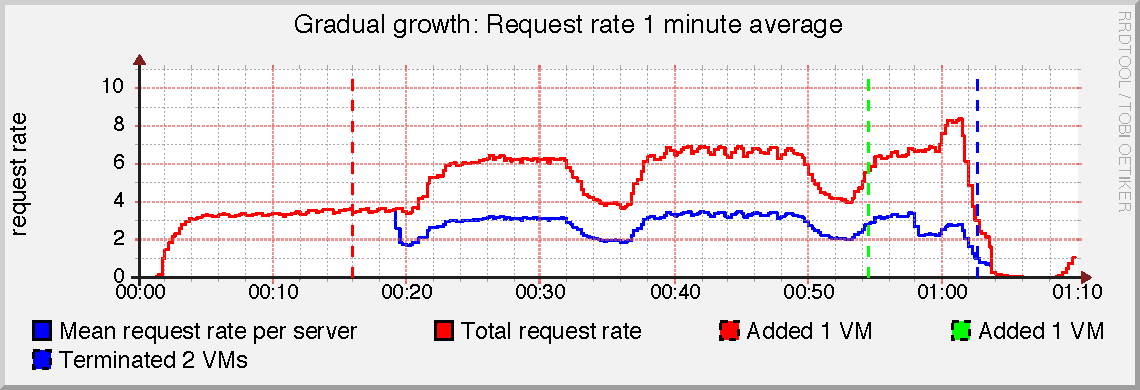
\includegraphics[width=\textwidth]{images/requestrategraph-test21}
	\caption{Request rate during test scenario 1}
	\label{fig:requestRateScenario1}
\end{figure}

\begin{figure}[htbp]
	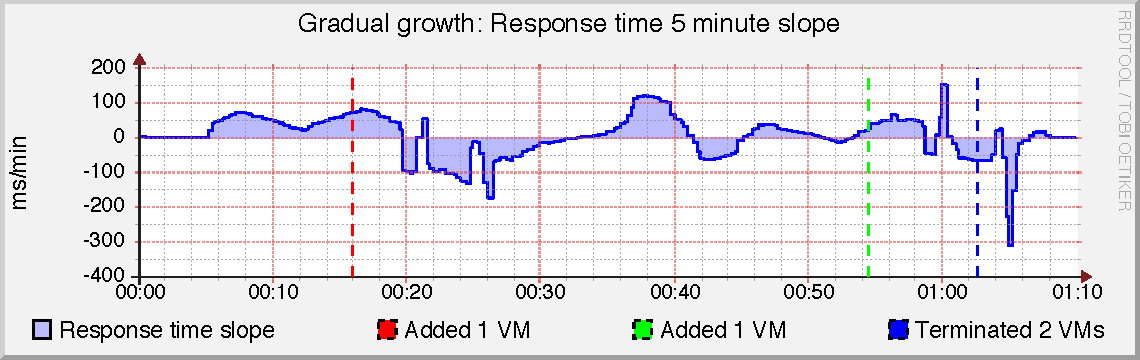
\includegraphics[width=\textwidth]{images/responsetimeslopegraph-test21}
	\caption{Response time slope during test scenario 1}
	\label{fig:responseTimeSlopeScenario1}
\end{figure}

\begin{figure}[htbp]
	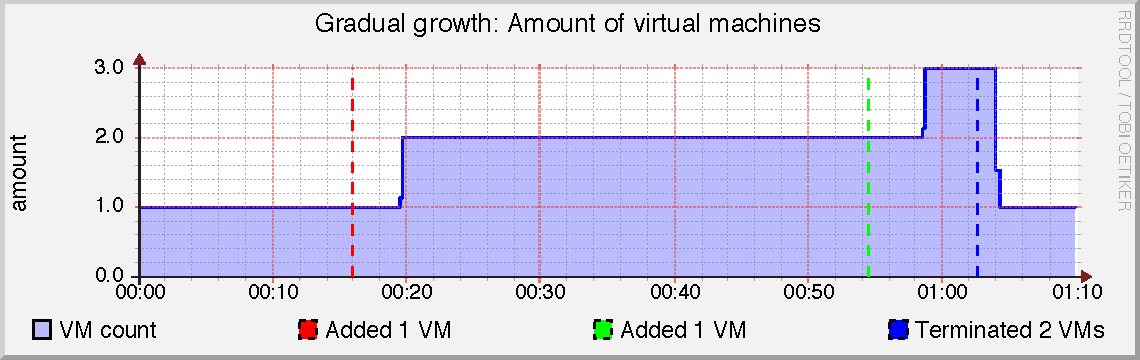
\includegraphics[width=\textwidth]{images/vmcountgraph-test21}
	\caption{Scaling utility during test scenario 1}
	\label{fig:vmCountScenario1}
\end{figure}

\begin{figure}[htbp]
	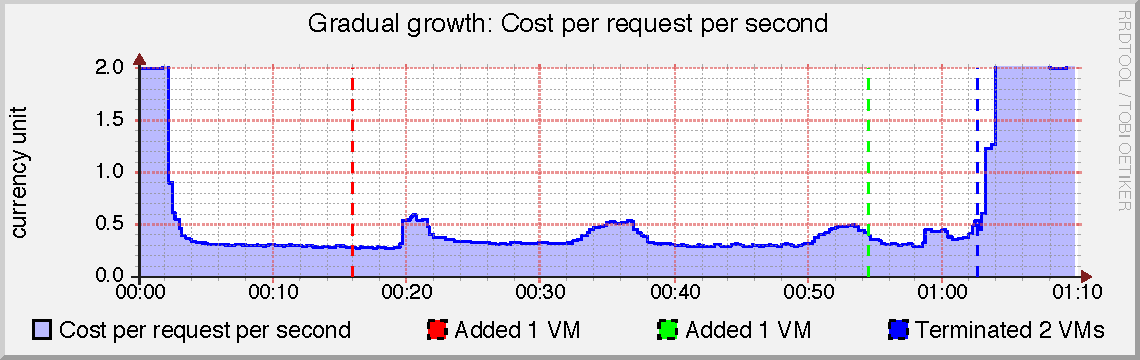
\includegraphics[width=\textwidth]{images/costperrequestpersecondgraph-test21}
	\caption{Cost per request per second during test scenario 1}
	\label{fig:costScenario1}
\end{figure}

\begin{figure}[htbp]
	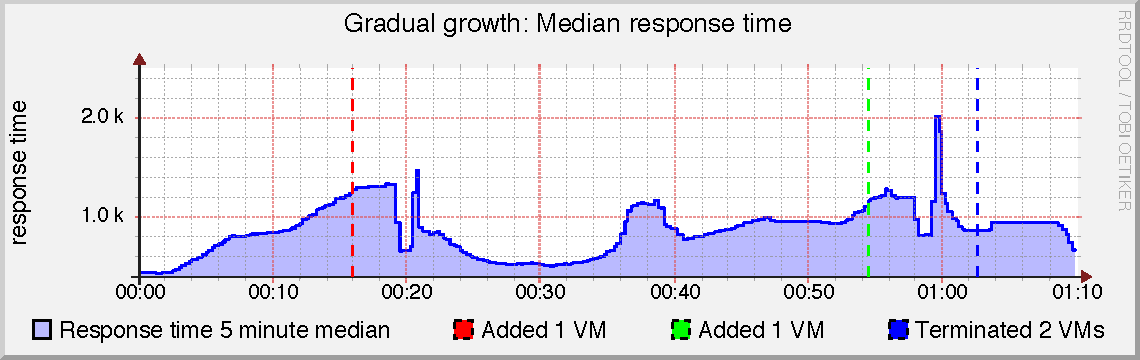
\includegraphics[width=\textwidth]{images/responsetimegraph-test21}
	\caption{Response time during test scenario 1}
	\label{fig:responseTimeScenario1}
\end{figure}

\begin{figure}[htbp]
	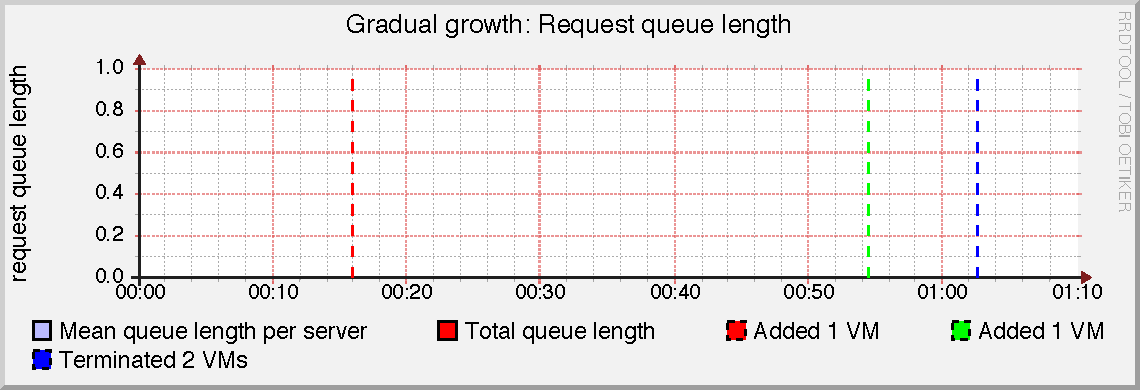
\includegraphics[width=\textwidth]{images/queuesizegraph-test21}
	\caption{Application server request queue size during test scenario 1}
	\label{fig:queueScenario1}
\end{figure}

\begin{figure}[htbp]
	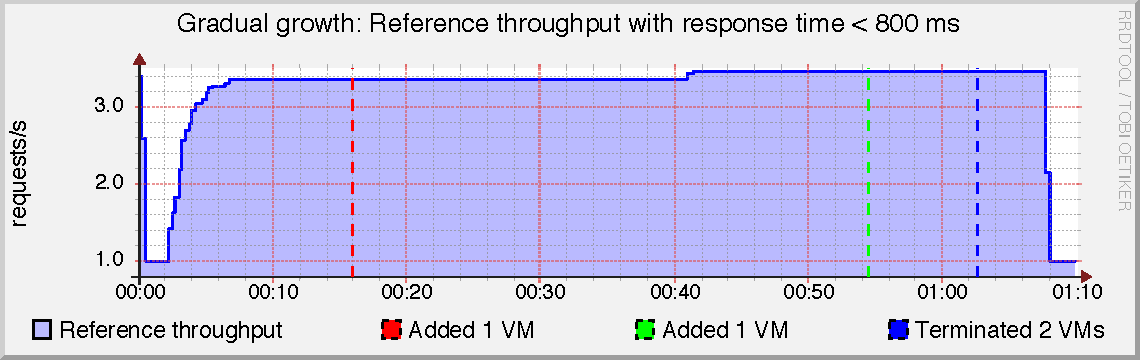
\includegraphics[width=\textwidth]{images/referencethroughputgraph-test21}
	\caption{Reference throughput during test scenario 1}
	\label{fig:referenceThroughputScenario1}
\end{figure}

\clearpage

\section{Figures for test scenario 2}

\begin{figure}[htbp]
	%\centering
	%\setlength\fboxsep{0pt}
	%\setlength\fboxrule{0.25pt}	
	%\centerline{
	%\hspace*{-3cm}
	%\rotatebox{90}{
	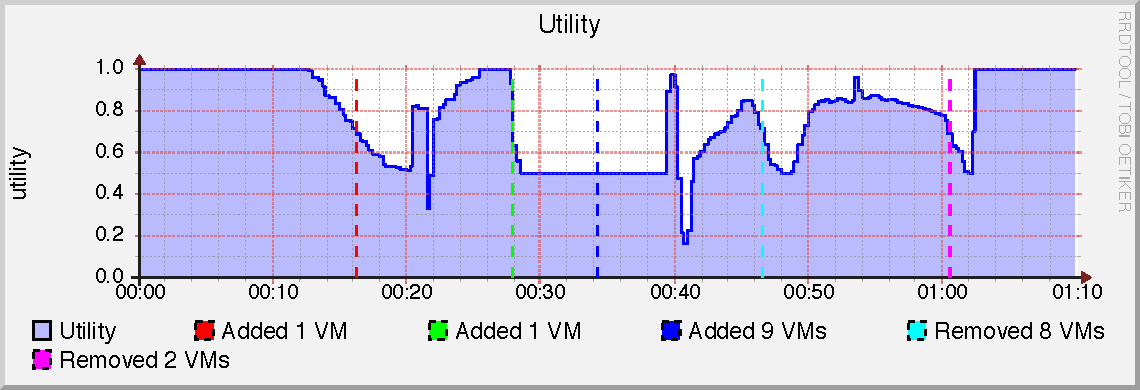
\includegraphics[width=\textwidth]{images/utilitygraph-test23}
	%}
	\caption{Utility during test scenario 2}
	\label{fig:utilityScenario2}
\end{figure}

\begin{figure}[htbp]
	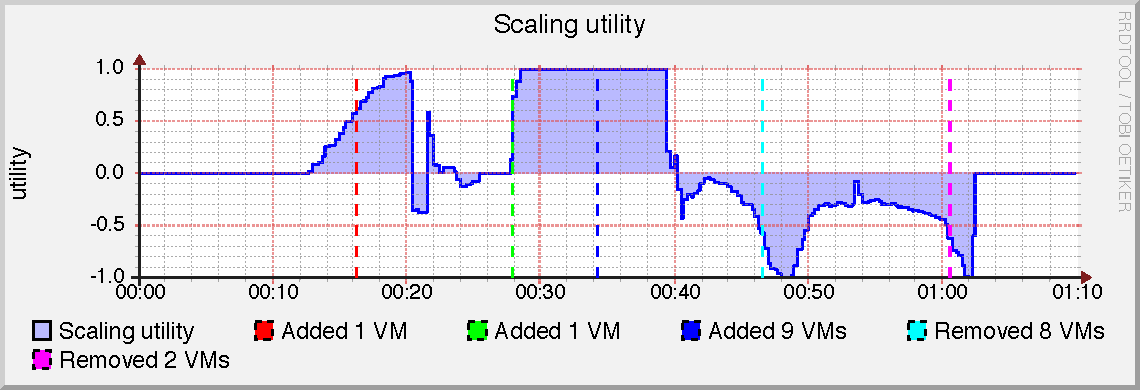
\includegraphics[width=\textwidth]{images/scalingutilitygraph-test23}
	\caption{Scaling utility during test scenario 2}
	\label{fig:scalingUtilityScenario2}
\end{figure}

\begin{figure}[htbp]
	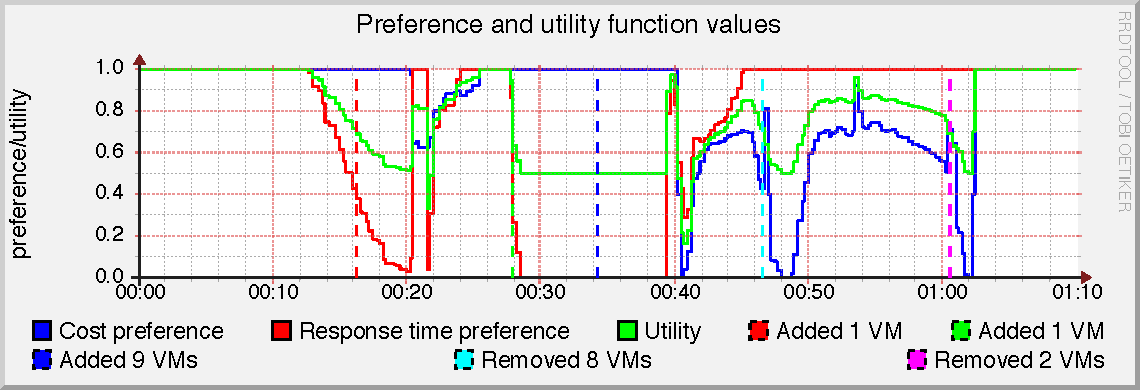
\includegraphics[width=\textwidth]{images/preferencesgraph-test23}
	\caption{Combined preference function and utility values during test scenario 2}
	\label{fig:preferencesScenario2}
\end{figure}

\begin{figure}[htbp]
	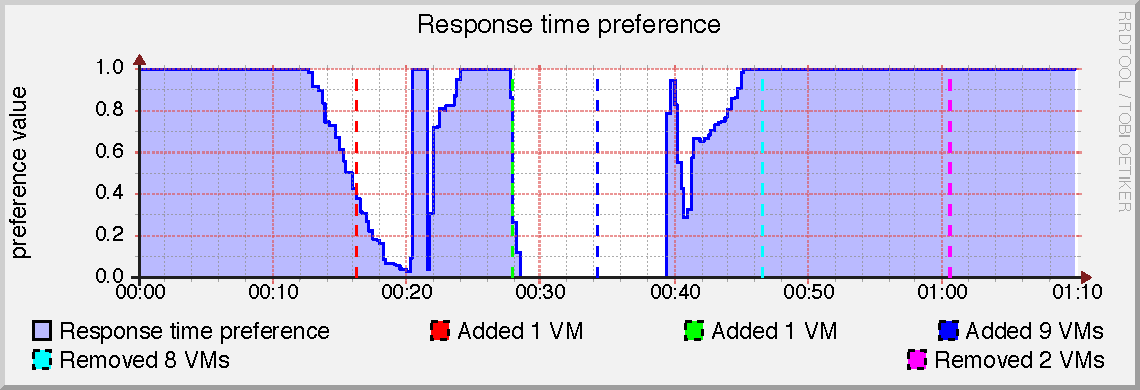
\includegraphics[width=\textwidth]{images/responsetimepreferencegraph-test23}
	\caption{Response time preference function values during test scenario 2}
	\label{fig:responseTimePreferenceScenario2}
\end{figure}

\begin{figure}[htbp]
	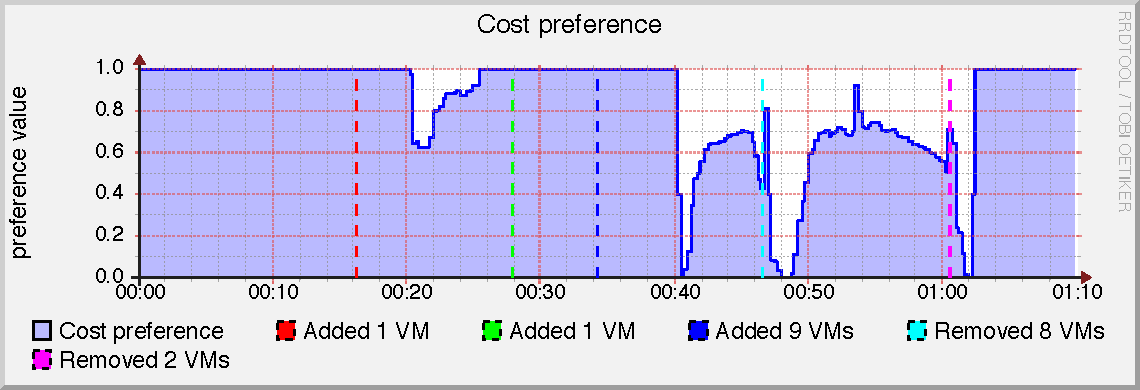
\includegraphics[width=\textwidth]{images/costpreferencegraph-test23}
	\caption{Cost preference function values during test scenario 2}
	\label{fig:costPreferenceScenario2}
\end{figure}

\begin{figure}[htbp]
	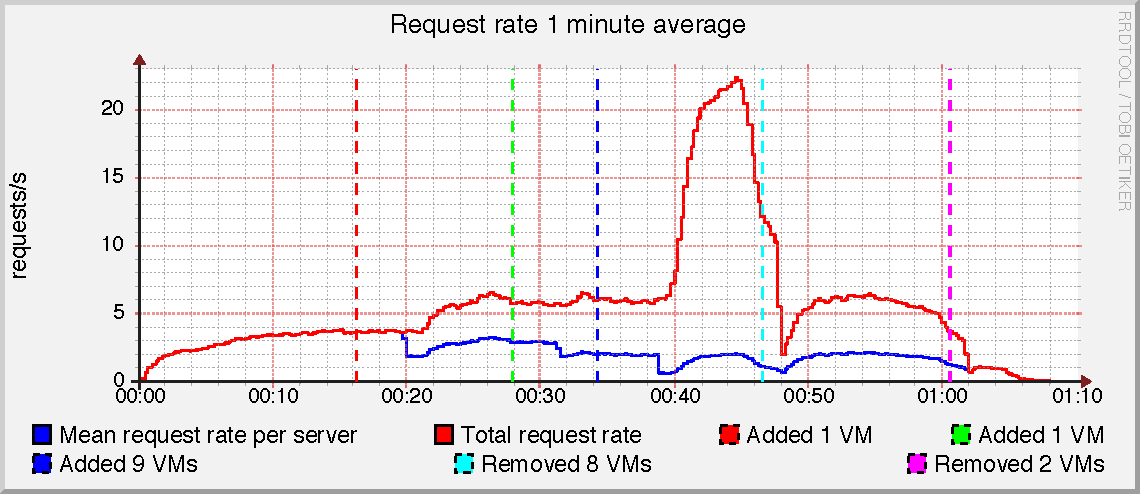
\includegraphics[width=\textwidth]{images/requestrategraph-test23}
	\caption{Request rate during test scenario 2}
	\label{fig:requestRateScenario2}
\end{figure}

\begin{figure}[htbp]
	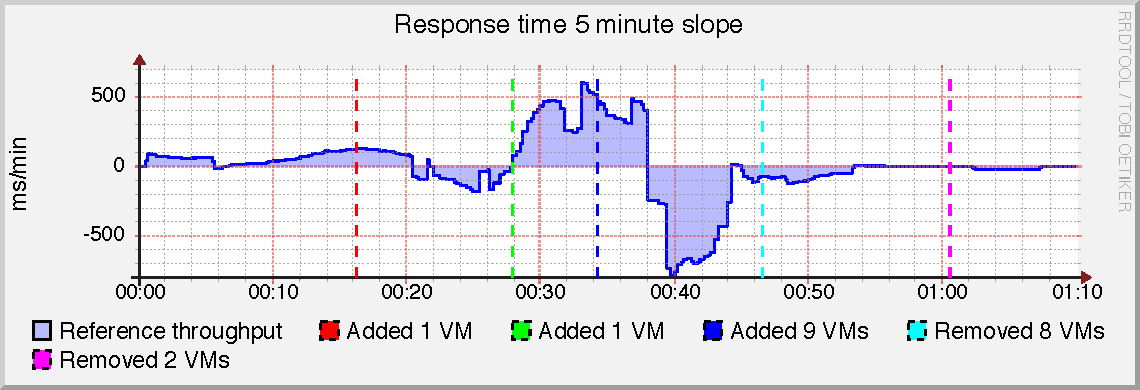
\includegraphics[width=\textwidth]{images/responsetimeslopegraph-test23}
	\caption{Response time slope during test scenario 2}
	\label{fig:responseTimeSlopeScenario2}
\end{figure}

\begin{figure}[htbp]
	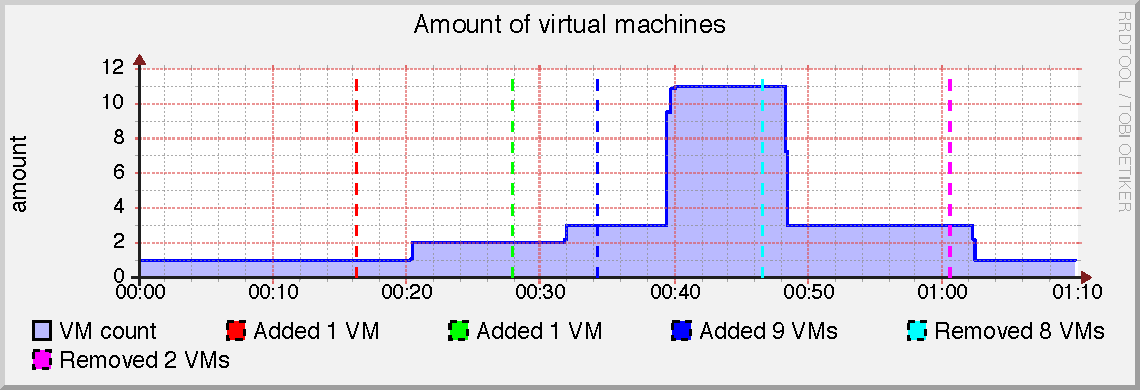
\includegraphics[width=\textwidth]{images/vmcountgraph-test23}
	\caption{Scaling utility during test scenario 2}
	\label{fig:vmCountScenario2}
\end{figure}

\begin{figure}[htbp]
	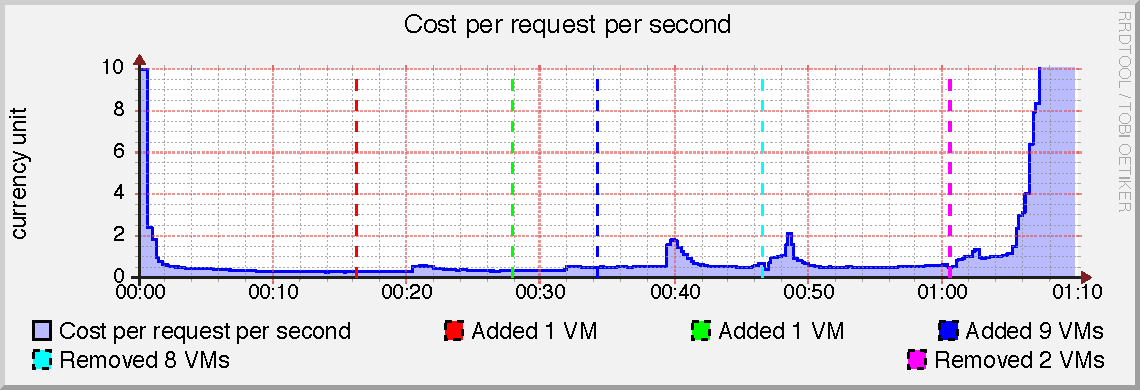
\includegraphics[width=\textwidth]{images/costperrequestpersecondgraph-test23}
	\caption{Cost per request per second during test scenario 2}
	\label{fig:costScenario2}
\end{figure}

\begin{figure}[htbp]
	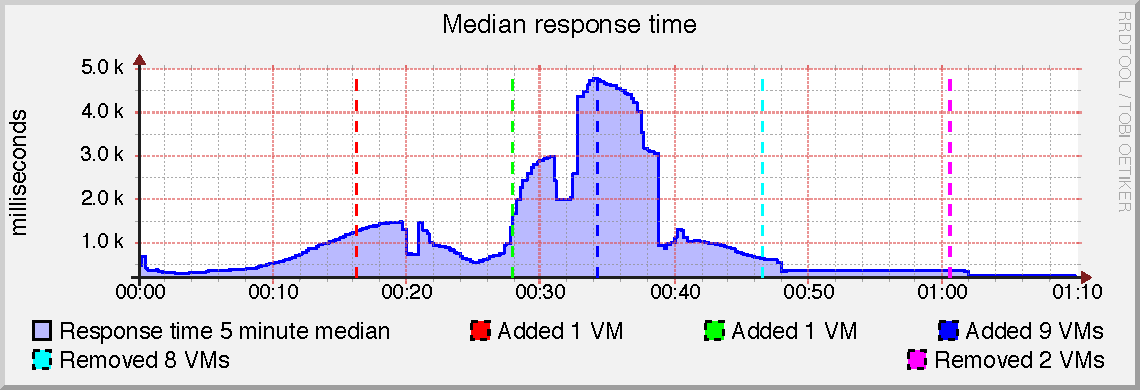
\includegraphics[width=\textwidth]{images/responsetimegraph-test23}
	\caption{Response time during test scenario 2}
	\label{fig:responseTimeScenario2}
\end{figure}

\begin{figure}[htbp]
	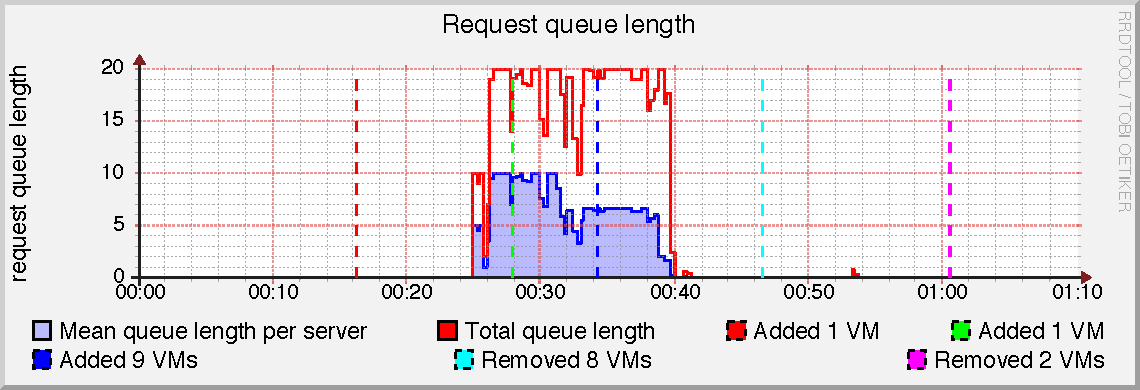
\includegraphics[width=\textwidth]{images/queuesizegraph-test23}
	\caption{Application server request queue size during test scenario 2}
	\label{fig:queueScenario2}
\end{figure}

\begin{figure}[htbp]
	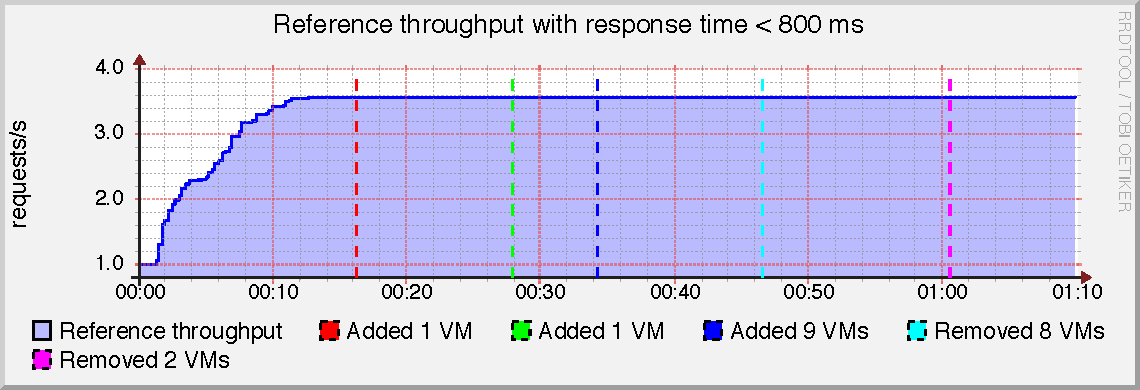
\includegraphics[width=\textwidth]{images/referencethroughputgraph-test23}
	\caption{Reference throughput during test scenario 2}
	\label{fig:referenceThroughputScenario2}
\end{figure}

\clearpage

% --- Back matter ---
%
% bibtex is used to generate the bibliography. The babplain style
% will generate numeric references (e.g. [1]) appropriate for theoretical
% computer science. If you need alphanumeric references (e.g [Tur90]), use
%
% \bibliographystyle{babalpha-lf}
%
% instead.

%\nocite{*}

\bibliographystyle{babplain-lf}
\bibliography{bibliography/ThesisStructure}


\end{document}


%Citing ~\cite{kilpelainen00}.


%\begin{figure}[h]
%%\begin{figure}[tbh] t= top, b = bottom, h=here
%\ \newline
%\begin{center}
%\includegraphics[width=0.9\textwidth]{kuvaesimerkki.pdf}
%%\rotatebox{90}{\includegraphics[scale=.75]{kuvaesimerkki.pdf}}
%\caption{Figure elements.}
%\label{kuvaesimerkki}
%\end{center}
%\end{figure}

% Attempt at pdf graph inclusion: 
% \begin{figure}[h]
% \centering
% 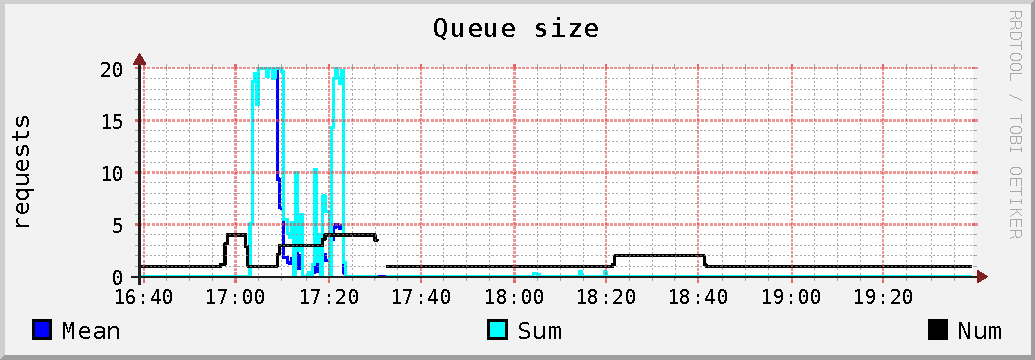
\includegraphics[width=0.8\textwidth]{images/meanvalue}
% \caption{Average queue size}
% \label{fig:meanvalue}
% \end{figure}